%----------------------------------------------------------------------------------------
%	PACKAGES AND OTHER DOCUMENT CONFIGURATIONS
%----------------------------------------------------------------------------------------

\documentclass[
 twoside=false % Leer el main.tex de la carpeta example para más opciones
]{kaobook}

% Set the language
\usepackage[spanish]{babel} % Load characters and hyphenation
\decimalpoint%
% \usepackage{adjustbox} % Para ajustar tablas
\usepackage[export]{adjustbox}
\usepackage{mathtools}
\usepackage[makeroom]{cancel}
% Load packages for testing
\usepackage{blindtext}

% \usepackage{tikzit}
\usetikzlibrary{babel}
\usetikzlibrary{quotes,angles}

% Load mathematical packages for theorems and related environments. 
%NOTE: choose only one between 'mdftheorems' and 'plaintheorems'.
\usepackage{styles/mdftheorems}
%\usepackage{styles/plaintheorems}

% Reset sidenote counter at chapters
%\counterwithin*{sidenote}{chapter}

\DeclareSymbolFont{yhlargesymbols}{OMX}{yhex}{m}{n}

\DeclareMathAccent{\widetriangle}{\mathord}{yhlargesymbols}{"E6}

\usepackage{draftwatermark}
\SetWatermarkText{Ludomatics}
\SetWatermarkAngle{45}
\SetWatermarkScale{0.5}
\SetWatermarkColor[gray]{0.96}

%----------------------------------------------------------------------------------------

\begin{document}

%----------------------------------------------------------------------------------------
%	BOOK INFORMATION
%----------------------------------------------------------------------------------------

\titlehead{Guía para ingreso a nivel superior}
\subject{Teoría y ejercicios}

\title[Guía para examen de admisión a nivel superior]{Guía para examen de admisión a nivel superior}
\subtitle{UNAM, IPN, UAM, ...}

\author[Ludomatics]{Ludomatics \thanks{Una empresa comprometida con tu educación}}

\date{\today}

\publishers{Auto publicado}

%----------------------------------------------------------------------------------------

% \frontmatter % Denotes the start of the pre-document content, uses roman numerals

%----------------------------------------------------------------------------------------
%	OPENING PAGE
%----------------------------------------------------------------------------------------

%\makeatletter
%\extratitle{
%	% In the title page, the title is vspaced by 9.5\baselineskip
%	\vspace*{9\baselineskip}
%	\vspace*{\parskip}
%	\begin{center}
%		% In the title page, \huge is set after the komafont for title
%		\usekomafont{title}\huge\@title
%	\end{center}
%}
%\makeatother

%----------------------------------------------------------------------------------------
%	COPYRIGHT PAGE
%----------------------------------------------------------------------------------------

% \makeatletter
% \uppertitleback{\@titlehead} % Header

% \lowertitleback{
% 	\textbf{Disclaimer}\\
% 	You can edit this page to suit your needs. For instance, here we have a no copyright statement, a colophon and some other information. This page is based on the corresponding page of Ken Arroyo Ohori's thesis, with minimal changes.
	
% 	\medskip
	
% 	\textbf{No copyright}\\
% 	\cczero\ This book is released into the public domain using the CC0 code. To the extent possible under law, I waive all copyright and related or neighbouring rights to this work.
	
% 	To view a copy of the CC0 code, visit: \\\url{http://creativecommons.org/publicdomain/zero/1.0/}
	
% 	\medskip
	
% 	\textbf{Colophon} \\
% 	This document was typeset with the help of \href{https://sourceforge.net/projects/koma-script/}{\KOMAScript} and \href{https://www.latex-project.org/}{\LaTeX} using the \href{https://github.com/fmarotta/kaobook/}{kaobook} class.
	
% 	The source code of this book is available at:\\\url{https://github.com/fmarotta/kaobook}
	
% 	(You are welcome to contribute!)
	
% 	\medskip
	
% 	\textbf{Publisher} \\
% 	First printed in May 2019 by \@publishers
% }
% \makeatother


%----------------------------------------------------------------------------------------
%	OUTPUT TITLE PAGE AND PREVIOUS
%----------------------------------------------------------------------------------------

% Note that \maketitle outputs the pages before here

% If twoside=false, \uppertitleback and \lowertitleback are not printed
% To overcome this issue, we set twoside=semi just before printing the title pages, and set it back to false just after the title pages
% \KOMAoptions{twoside=semi}
% \maketitle
% \KOMAoptions{twoside=false}

%----------------------------------------------------------------------------------------
%	MAIN BODY
%----------------------------------------------------------------------------------------

\mainmatter % Denotes the start of the main document content, resets page numbering and uses arabic numbers
\setchapterstyle{kao} % Choose the default chapter heading style

% \pagelayout{wide} % No margins
% \addpart{Matemáticas}
% \pagelayout{margin} % Restore margins
% \graphicspath{{materias/matematicas/aritmetica/assets/}}

\setchapterimage[5.5cm]{bg03}
%https://www.123rf.com/stock-photo/trigonometry.html?sti=mwt5gbafw3l7clx5s6|
%&mediapopup=49203529
\chapter{Aritmética}
\labch{aritmetica}
\section{Introducción}
\blindtext


% \graphicspath{{materias/matematicas/algebra/assets/}}

\setchapterimage[5.5cm]{bg03}
%https://www.123rf.com/stock-photo/trigonometry.html?sti=mwt5gbafw3l7clx5s6|
%&mediapopup=49203529
\chapter{Álgebra}
\labch{algebra}
\section{Introducción}
\blindtext


\graphicspath{
  {materias/matematicas/trigonometria/assets/}
  {materias/matematicas/trigonometria/ejercicios/}
}

% \setchapterimage[5.5cm]{bg03}
%https://www.123rf.com/stock-photo/trigonometry.html?sti=mwt5gbafw3l7clx5s6|
%&mediapopup=49203529
\chapter{Trigonometria}
\labch{trigonometrica}
\section{Introducción}
La \textbf{trigonometría} se dedica al estudio de las medidas de los triángulos 
y su relación entre ellas.
Dichas medidas son básicamente:
\begin{itemize}
  \item Lados y
  \item Ángulos
\end{itemize}

Por otra parte, un \textbf{triángulo} se define como una figura plana de tres 
lados. Además de los lados y los ángulos, un triángulo presenta una tercera 
propiedad llamada \textit{vértice}.
Los \textbf{vértices} son simplemente puntos que se unen mediante segmentos de recta para
poder formar un triángulo.

\begin{marginfigure}[-3.5cm]
	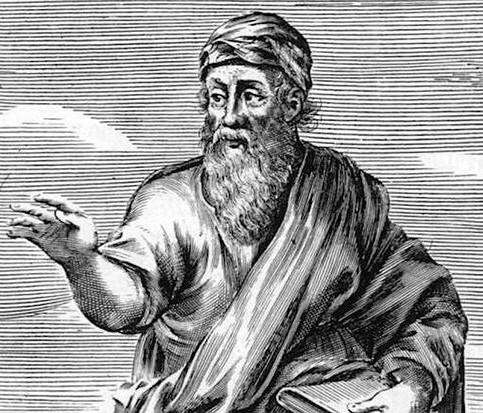
\includegraphics{pythagoras_cropped}
	\caption[pythagoras]{Pitágoras. Filósofo y matemático griego distinguido por 
    sus aportaciones a la artimética, geometría y trigonometría.
    % \\ 
	  % \url{https://www.pinterest.com/pin/133841420159654763/}
  }
	\labfig{pythagoras}
\end{marginfigure}

\subsection{Notación para nombrar triángulos}

Un triángulo puede ser nombrado con ayuda de sus vértices, de esta manera el 
triángulo de la figura \reffig{triangulo} se denota como el triángulo ABC que se 
representa como:
$$\widetriangle{ABC}$$

\begin{figure}[hb]
	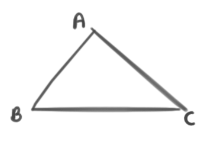
\includegraphics[width=0.40\textwidth]{triangulo}
	\caption[Triangulo]{Triángulo ABC. }
	\labfig{triangulo}
\end{figure}

\paragraph{Aspectos interesantes de la trigonometría}
\begin{itemize}
  \item Es una de las ramas de la matemática más antigua, su estudio se remonta 
  a la época griega en donde su exponente principal fue \textit{Pitágoras}, pese 
  a que oficialmente se reconozca a \textit{Hiparco de Nicea} como el padre de 
  la trigonometría.

  \item Los triángulos son los polígonos más simples
  \begin{itemize}
    \item Por ende carecen de diagonales
  \end{itemize}

  \item Para el estudio de otros polígonos se suele utilizar el método de 
  \textit{triángulación}, que se refiere básicamente a dividir dicha figura en 
  un conjunto ordenado de triángulos.
  %TODO:- Agregar la etimologia
\end{itemize}

% pseudo referencias 
% https://concepto.de/triangulo/
\section{Ángulos}
\subsection{¿Qué es un ángulo?}

\begin{definition}
	Un \textbf{ángulo} se define como la abertura (o región del plano) 
	comprendida entre los semirectas que tienen un origen en común, 
	llamado \textit{vértice}
\end{definition}

\begin{figure}[hb]
	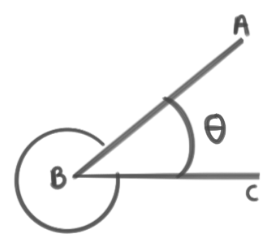
\includegraphics[width=0.40\textwidth]{angulo}
	\caption[Angulo]{Ángulo ABC. En donde:
	\begin{itemize}
		\item \textbf{B} es el vértice del ángulo
		\item $\pmb{\overline{BC}}$ es el lado inicial del ángulo
		\item $\pmb{\overline{BA}}$ es el lado final o terminal del ángulo
	\end{itemize} }
	\labfig{angulo}
\end{figure}

\marginnote[2mm]{$\pmb{\overline{BA}}$ se lee como el segmento BA}

\begin{itemize}
	\item De manera gráfica un ángulo se representa mediante un arco de 
	circunferencia.

	\item Es importante destacar que las dos semirectas siempre formarán 
	\textit{dos ángulos}:
	
	\begin{itemize}
		\item Un ángulo \textbf{interno} y
		\item Un ángulo \textbf{externo}
	\end{itemize}

	\item Por último, si juntamos (sumamos) el ángulo \textbf{interno} y 
	el \textbf{externo} obtendremos una vuelta, mejor conocida como 
	\textbf{revolución}

\end{itemize}

Otras consideraciones importantes para trabajar con ángulos son que:

\begin{itemize}
	\item La simbología para representar ángulos es variada, se sueleve usar: 
	$\pmb{\angle,\; \measuredangle}$, $\angle\; A$, $\hat{a}$
	\begin{itemize}
		\item También se suele utilizar la notación $\pmb{\angle ABC}$
		\item De la cual se debe entender que la letra de en medio representa el 
		vértice del ángulo al que se hace referencia.
	\end{itemize}
	\item Tamién es posible representar los ángulos con letras griegas,
	por ejemplo: $\pmb{\alpha,\; \beta,\; \gamma,\; ...}$
	%TODO:- Agregar más colores
	\item \textbf{Si el ángulo se mide en sentido \textit{contrario a las 
	manecillas del reloj}, entonces es \textit{positivo}}.
	\sidenote[][-6cm]{\textbf{Ángulo positivo}\\ 
	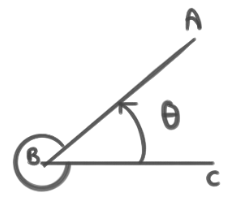
\includegraphics[width=3.5cm]{angpos}}
	\item \textbf{Si el ángulo se mide en sentido \textit{de las 
	manecillas del reloj}, entonces es \textit{negativo}}.
	\sidenote[][-2cm]{\textbf{Ángulo negativo}\\ 
	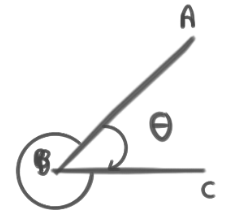
\includegraphics[width=3.5cm]{angneg}}
\end{itemize}

\subsection{Clasificación de ángulos}

\subsubsection{Primera clasificación}

Los ángulos pueden ser clasificados de acuerdo a su medida como se muestra en la
tabla \ref{clasifangulos}.

\begin{figure*}[h!]
% \begin{adjustbox}{max width=16.3cm}
\def\arraystretch{1.5}%  1 is the default, change whatever you need
\caption[Clasificación de ángulos]{Clasificación de ángulos. 
	Se toma como base su medida
}
%TODO:- Corregir referencia de la tabla.
\labtab{clasifangulos}
\label{clasifangulos}
\begin{tabular}{c | c | c }
	% \hline
	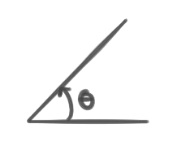
\includegraphics[width=4cm]{agudo} & 
	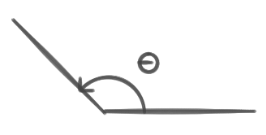
\includegraphics[width=4cm]{obtuso}  & 
	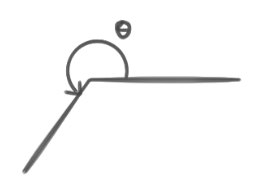
\includegraphics[width=4cm]{entrante} 
	\\ %\hline

	\textbf{Agudo} & 
	\textbf{Obtuso} & 
	\textbf{Entrante}                       
	\\ %\hline

	$0^\circ < \theta < 90^\circ$ &
	$90^\circ < \theta < 180^\circ$ &
	$180^\circ < \theta < 360^\circ$ 
	\\

	\parbox{4cm}{
		\begin{center}
			Mayores que $0^\circ$ y \\ Menores que $90^\circ$
		\end{center} 
	} & 
	\parbox{4cm}{
		\begin{center}
			Mayores que $90^\circ$ y \\ Menores que $180^\circ$
		\end{center} 
	} & 
	\parbox{4cm}{
		\begin{center}
			Mayores que $180^\circ$ y \\ Menores que $360^\circ$
		\end{center} 
	}                                 
	\\ \hline

	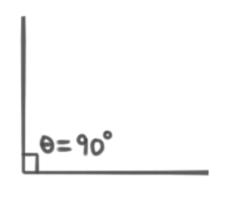
\includegraphics[width=4cm]{recto} & 
	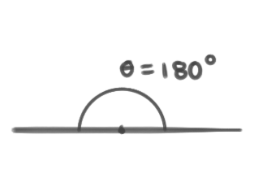
\includegraphics[width=4cm]{llano} & 
	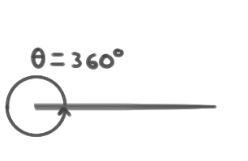
\includegraphics[width=4cm]{perigonal} 
	\\ %\hline
	\textbf{Recto} & 
	\textbf{Llano}  & 
	\textbf{Perigonal o de vuelta completa} 
		\\ %\hline

	$\theta = 90^\circ$ &
	$\theta = 180^\circ$ &
	$\theta = 360^\circ$ 
	\\

	\parbox{4cm}{
		\begin{center}
			Exactamente $90^\circ$
		\end{center} 
	} & 
	\parbox{4cm}{
		\begin{center}
			Exactamente $180^\circ$
		\end{center} 
	} & 
	\parbox{4cm}{
		\begin{center}
			Exactamente $360^\circ$
		\end{center} 
	}                                 
	% \\ \hline
\end{tabular}
% \end{adjustbox}
\end{figure*}

\subsubsection{Segunda clasificación}

La segunda clasificación de ángulos hace uso del concepto de ángulo 
\textit{recto}, \textit{llano} y \textit{perigonal}. Dicha clasificación se 
da siempre para dos o más ángulos a través del concepto de completariedad y 
sumplementaridad como se ve a continuación.


\begin{figure*}[h!]
% \begin{adjustbox}{max width=16.3cm}
\def\arraystretch{1.5}%  1 is the default, change whatever you need
\caption[Clasificación de ángulos]{Segunda clasificación de ángulos. 
	Se toma como base su la completariedad o sumplementaridad entre ellos.
}
%TODO:- Corregir referencia de la tabla.
\labtab{clasifangulosdos}
\label{clasifangulosdos}
\begin{tabular}{c | c | c }
	% \hline
	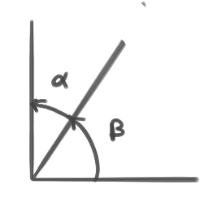
\includegraphics[width=4cm]{complementario} & 
	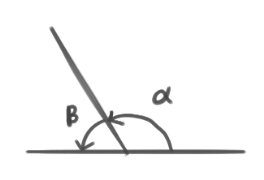
\includegraphics[width=4cm]{suplementario}  & 
	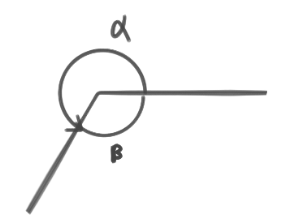
\includegraphics[width=4cm]{conjugado} 
	\\ %\hline

	\textbf{Ángulos complementarios} & 
	\textbf{Ángulos suplementarios} & 
	\textbf{Ángulos conjugados}                       
	\\ %\hline

	$\angle \alpha + \angle \beta= 90^\circ$ &
	$\angle \alpha + \angle \beta= 180^\circ$ &
	$\angle \alpha + \angle \beta= 360^\circ$ 
	\\

	\parbox{4cm}{
		\begin{center}
			La suma de los ángulos tiene que dar exactamente $90^\circ$
		\end{center} 
	} & 
	\parbox{4cm}{
		\begin{center}
			La suma de los ángulos tiene que dar exactamente $180^\circ$
		\end{center} 
	} & 
	\parbox{4cm}{
		\begin{center}
			La suma de los ángulos tiene que dar exactamente $360^\circ$
		\end{center} 
	}                                 

\end{tabular}
% \end{adjustbox}
\end{figure*}

%TODO:- Agregar ejemplos
\begin{figure*}[h!]
 \begin{kaoexercises}
	Hallar el valor de todos los ángulos en las siguientes figuras
  \begin{multicols}{3}
		\begin{enumerate}[itemsep=2pt,parsep=2pt]
			% 1
			\item \textbf{}\\
			\input{materias/matematicas/trigonometria/actividades/act_01/01}
			
			% 2
			\item \textbf{}\\
			\input{materias/matematicas/trigonometria/actividades/act_01/02}
			
			% 3
			\item \textbf{}\\
			\input{materias/matematicas/trigonometria/actividades/act_01/03}

			% 4
			\item \textbf{} \\
			\input{materias/matematicas/trigonometria/actividades/act_01/04}
			\columnbreak%

			% 5
			\item \textbf{} \\
			\input{materias/matematicas/trigonometria/actividades/act_01/05}

			% 6
			\item \textbf{}\\	
			\input{materias/matematicas/trigonometria/actividades/act_01/06}

			% 7
			\item \textbf{} \\
			\input{materias/matematicas/trigonometria/actividades/act_01/07}
			\columnbreak%

			% 8
			\item \textbf{}\\
			\input{materias/matematicas/trigonometria/actividades/act_01/08}

			% 9
			\item \textbf{}\\
			\input{materias/matematicas/trigonometria/actividades/act_01/09}	

			% 10
			\item \textbf{} \\
			\input{materias/matematicas/trigonometria/actividades/act_01/10}				

		\end{enumerate}
  \end{multicols}
\end{kaoexercises}
\end{figure*}

\subsection{Sistema de medición de ángulos}

Para expresar la medida de lo ángulos contamos con dos sistemas de medición.

\subsubsection{Sistema sexagesimal}

El sistema sexagesimal es un sistema de numeración de base 60 que se usaba en 
la antigüedad para medir tiempos (lo que ahora conocemos como horas, minutos y
segundos). Además, tiene la ventaja de tener muchos divisores por lo que 
hacer proporciones (comparaciones) entre cantidades, era relativamente sencillo.
En consecuencia, también fue utilzado para medir ángulos, partiendo de la idea 
de relacionarlo con el tiempo.

Así mismo, a la idea de relacionar la medida de los ángulos con el tiempo se le 
suma el hecho de que la circunferencia se divide en 360 partes, llamadas 
\textbf{grados} \sidenote[][-2.5cm]{Se representa con el símbolo $\circ$, por ejemplo,
$45^\circ$}.
\begin{itemize}
	\item El grado se parte en 60 partes llamadas \textbf{minutos}
	\sidenote[][-2.3cm]{Los minutos se representan con un apostrófe ('), por ejemplo,
	$45'$, se lee 45 minutos} 
	y
	\item El minuto se parte en 60 partes llamadas \textbf{segundos}
	\sidenote[][-1.6cm]{Los segundos se representan con dos apostrófes (''), por ejemplo,
	$27'$, se lee 27 segundos}.
\end{itemize}

\marginnote[-5mm]{En el sistema sexagesimal podemos tener la medida del ángulo
como una combinación de grados, minutos y segundos. 
Por ejemplo $34^\circ\; 27'\; 45''$. 
Lo anterior se lee como: ``34 grados, 27 minutos, 45 segundos''}

De esta manera surgen las siguientes equivalencias:

\begin{equation*}
\boxed{
\begin{array}{rcl}	
		1\; rev &=& 360^\circ \\
		1^\circ &=& 60\;' \\
		1\;' &=& 60\;'' 
	\end{array}
}
\end{equation*}

\subsubsection{Conversiones entre grados, minutos y segundos}
Para hacer la conversión de grados a minutos o de minutos a segundos basta con 
relacionarlos mediante una regla de tres. Sin embargo el esquema (REF) ilustra
una forma más fácil. 

\begin{figure}[hb]
	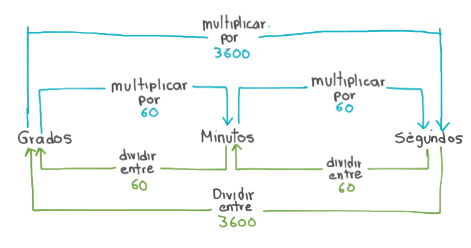
\includegraphics[width=\textwidth]{conversiongms}
	\caption[conversiongms]{Conversión entre grados, minutos y segundos.}
	\labfig{conversiongms}
\end{figure}

Veamos algunos ejemplos.

\begin{example}
	Convertir $\pmb{30^\circ\; 27'\; 38''}$ a Grados. \\
	\begin{enumerate}
		\item El primer paso consiste en transformar los minutos a grados. 
		Para ello:
		\begin{equation*}
			\dfrac{27'}{60} = 0.45^\circ
		\end{equation*}

		\item Luego, debemos de pasar los segundos a grados. Para ello: 
		\begin{equation*}
			\dfrac{38'}{3600} = 0.0105^\circ
		\end{equation*}

		\item Por último, como todas las cantidades están en la misma unidad, solo 
		queda sumarlas.
		\begin{align*}
			30^\circ\; 27'\; 38'' &= 30^\circ\; +\; 0.45^\circ\; +\; 0.0105^\circ \\
			\Aboxed{\pmb{30^\circ\; 27'\; 38''} &= 30.4605^\circ}
		\end{align*}

	\end{enumerate}
\end{example}

\begin{example}
	Convertir $\pmb{62.972^\circ}$ a grados y minutos
	\begin{enumerate}
		\item Lo primero que tenemos que hacer es descomponer $62.972^\circ$ en la 
		parte entera y la parte decimal. \\
		La parte entera ya se encuentra en grados por lo cual no hay nada más que 
		hacer.

		\item La parte decimal ($0.972^\circ$) la podemos transformar a minutos.
		Para ello, como lo indica el esquema \reffig{conversiongms}, debemos 
		\textbf{multiplicar por 60}
		\begin{equation*}
			0.972^\circ \times 60 = 58.32' 
		\end{equation*}

		\item Por último, se unen los grados y los minutos, de manera que nos queda 
		como: 
		\begin{equation*}
			\boxed{\pmb{62.972^\circ} = 62^\circ\; 58.32'}
		\end{equation*}
	\end{enumerate}
\end{example}

\begin{example}
	¿Qué pasa si nos piden convertir la cantidad anterior ($\pmb{62.972^\circ}$) a
	grados, minutos y segundos?
	\begin{enumerate}
		\item Debemos pasar la parte decimal ($.972^\circ$) a minutos.\\
		Lo cual da como resultado: $58.32'$.

		\item Ahora, la parte decimal de lo minutos ($0.32'$) debemos pasarla a 
		segundos. Para ello \textbf{multiplicamos por 60}:
		\begin{equation*}
			0.32 \times\ 60 = 19.2''
		\end{equation*}

		\item Por último, se unen los grados, minutos y segundos de la siguiente 
		forma:
		\begin{equation*}
			\boxed{\pmb{62.972^\circ} = 62^\circ\; 58'\; 19.2''}
		\end{equation*}
	\end{enumerate}
\end{example}

\begin{figure*}[h!]
 \begin{kaoexercises}
 Convierte los siguientes ángulos a \textit{solo} grados
 \begin{multicols}{4}
		\begin{enumerate}
		\setlength\itemsep{4mm}
		\item $40^\circ 10' 15''$
		\item $61^\circ 42' 21''$
		\item $1^\circ 2' 3''$
		\item $73^\circ 40' 40''$
		\item $9^\circ 9' 9''$
		\item $98^\circ 22' 45''$
		\item $23^\circ 24' 25''$
		\item $320^\circ 20' 17''$
		\item $322^\circ 50' 59''$
		\item $9^\circ 2' 1''$
	\end{enumerate}
 \end{multicols}

 Convierte los siguientes ángulos a su equivalente en grados, minutos y segundos.
 \begin{multicols}{4}
		\begin{enumerate}
		\setlength\itemsep{4mm}
		\item $40.32^\circ$
		\item $61.24^\circ$
		\item $18.255^\circ$
		\item $29.411^\circ$
		\item $19.99^\circ$
		\item $44.01^\circ$
		\item $32.123^\circ$
		\item $34.98^\circ$
		\item $32.29^\circ$
		\item $769^\circ$
	\end{enumerate}
 \end{multicols}

 \end{kaoexercises}
\end{figure*}

\subsubsection{Operaciones con ángulos}

Al igual que con los números arábicos, se pueden realizar las operaciones 
básicas con los ángulos en el sistema sexagesimal. A continuación veremos 
ejemplos de cómo realizar la suma, resta, multiplicación y división.\\

%TODO:- Revisar explicacion
Para realizar dichas operaciones basta con recordar dos cosas:
\begin{itemize}
	\item ``Peras con peras, manzanas con manzanas'', es decir, se deben operar
	grados con grados, minutos con minutos y segundos con segundos.

	\item Normalmente estamos acostumbrados a realizar operaciones en un sistema 
	decimal, es decir, base 10, pero, ¿Cómo realizariamos operaciones en un 
	sistema sexagesimal (base 60)?
	\begin{itemize}
		\item Analicemos que pasa en una suma en sistema decimal\\
		\begin{center}
			\begin{tabular}{c c c c}
				& \textcolor{red}{\pmb{1}}  & \textcolor{blue}{\pmb{1}} & \\
				& 4 & 3 & 4 \\
			+ &   & 9 & 8 \\
			\hline
				& 5 & 3 & 2 \\
			\end{tabular}
		\end{center}

		\begin{itemize}
			\item El máximo número que podemos poner es $9$ (el número anterior 
			a la base).
			\item Si el resultado de la suma de los primeros términos es mayor a $9$
			entonces solo se pone la unidad y la decena se pasa a la siguiente 
			posición.\\
			De esta manera, $4 + 8 = 12$, por lo tanto se pone el $2$ y el $1$ que
			representa las decinas se pasa a la siguiente posición.\\
			Este proceso se repite hasta que las se hayan recorrido todas las 
			posiciones de izquierda a derecha.
		\end{itemize}

		\item Ahora, intentemos realizar una operación en una \textbf{pseudo-base}
		\sidenote{Para que realmente fuera base 60 se necesitan 60 símbolos
		completamente distintos, cada uno representando una posición en la recta 
		númerica.\\ Por ejemplo un sistema base 2 solo tiene dos símbolos: $0$ y $1$
		} 60.

		\begin{center}
			\begin{tabular}{c c c c}
					& 40 & 38 & 12 \\
				+ &   & 49 & 47 \\
				\hline
			\end{tabular}
		\end{center}

		\begin{itemize}
			\item Debemos resolver de izquierda a derecha como en la suma con numeros 
			decimales
			\item El máximo número que podemos poner es 59 (uno antes que la base)
			\item Por lo tanto, $12 + 47 = \textcolor{orange}{59}$
			\begin{center}
				\begin{tabular}{c c c c}
						& 40 & 38 & 12 \\
					+ &   & 49 & 47 \\
					\hline
					& 		&    & \textcolor{orange}{59}
				\end{tabular}
			\end{center}

			\item Repetimos el mismo proceso para la siguiente posición: $38 + 49=87$,
			sin embargo, $87$ se puede expresar como $\textcolor{blue}{60} + 
			\textcolor{orange}{37}$. Por lo tanto podemos hacer lo siguiente:
			\begin{center}
				\begin{tabular}{c c c c}
						&\textcolor{blue}{60} & & \\
						& 40 & 38 & 12 \\
					+ &   & 49 & 47 \\
					\hline
					& 		& \textcolor{orange}{37}   & 59
				\end{tabular}
			\end{center}

			\item Una vez más hacemos lo mismo para $\textcolor{orange}{60} + 
			\textcolor{blue}{40} = 100$. Sin embargo no podemos escribir $100$ por lo 
			que dejamos los mismo números, por lo tanto queda como:
			\begin{center}
				\begin{tabular}{c c c c c}
						&\textcolor{blue}{60}& & & \\
						&& 40 & 38 & 12 \\
					+ &&   & 49 & 47 \\
					\hline
					& & \textcolor{orange}{40}		& 37   & 59
				\end{tabular}
			\end{center}

			\item Como 60 no tiene con quién sumarse simplemente lo 
			descomponemos como $\textcolor{orange}{59} + \textcolor{orange}{1}$, 
			porque el máximo número que podemos colocar
			es $59$. 
			\begin{center}
				\begin{tabular}{c c c c c c}
						&\textcolor{blue}{1}&& & & \\
						&&& 40 & 38 & 12 \\
					+ &&&   & 49 & 47 \\
					\hline
					&&\textcolor{orange}{59} & 40		& 37   & 59
				\end{tabular}
			\end{center}

			\item Por último, cómo $1$ no tiene con quién operarse simplemente lo 
			bajamos.
			\begin{center}
				\begin{tabular}{c c c c c c}
						&&& & & \\
						&&& 40 & 38 & 12 \\
					+ &&&   & 49 & 47 \\
					\hline
					&1&59 & 40		& 37   & 59
				\end{tabular}
			\end{center}
		\end{itemize}
	\end{itemize}

	\item Realizar operaciones con ángulos es más sencillo que el ejemplo 
	anterior debido a que tenemos el concepto de grado, minuto y segundo y sus 
	correspondentes equivalencias.
\end{itemize}

Veamos un ejemplo de cada operación:
\paragraph{Suma}

\begin{example}
	Realizar la siguiente operación:
		$39^\circ\; 48'\; 54'' + 18^\circ\; 23'\; 49'' $
	\begin{itemize}
		\item El primer paso es sumar los segundos. $54'' + 49'' = 103$. $103$ puede 
		ser reescrito como $\textcolor{blue}{60''} + \textcolor{orange}{43''}$. \\
		Además, $\textcolor{blue}{60''} = \textcolor{blue}{1'}$.
		\begin{center}
			\begin{tabular}{ c c c c}
					& & $\textcolor{blue}{1'}$ & \\
					& $39^\circ$ & $48'$ & $54''$ \\
				+ & $18^\circ$  & $23'$ & $49''$ \\
				\hline
				&  &   & $\textcolor{orange}{43''}$
			\end{tabular}
		\end{center}		

		\item Se repite el mismo proceso de tal manera que: $1' +'48' + 23' = 72'$.
		$72' = \textcolor{blue}{1^\circ} + \textcolor{orange}{12'}$
		\begin{center}
			\begin{tabular}{ c c c c}
					& $\textcolor{blue}{1^\circ}$ & $\textcolor{gray}{1'}$ & \\
					& $39^\circ$ & $48'$ & $54''$ \\
				+ & $18^\circ$  & $23'$ & $49''$ \\
				\hline
				&  & $\textcolor{orange}{12'}$   &$43''$
			\end{tabular}
		\end{center}	

		\item Finalmente, para los grados no es necesario pensar en términos de base 
		60, por lo que simplemente se suman sin importar que el valor sea mayor a 
		59.
		\begin{center}
			\begin{tabular}{ c c c c}
					& $39^\circ$ & $48'$ & $54''$ \\
				+ & $18^\circ$  & $23'$ & $49''$ \\
				\hline
				& $\textcolor{orange}{58^\circ}$ & $12'$   &$43''$
			\end{tabular}
		\end{center}	
	\end{itemize}
\end{example}

\paragraph{Resta}
La operación de resta o diferencia se realiza igual que en el sistema decimal y 
también se utiliza la clásica expresión de ``pedir prestado al número del lado 
izquierdo''.
\begin{example}
	Realizar la siguiente operación:
	$39^\circ\; 18'\; 34'' - 18^\circ\; 23'\; 49'' $
	\begin{itemize}
		\item Cómo $49''$ (sustraendo) es mayor que el $34''$ (minuendo) debemos
		``pedir préstamo'' al número de al lado. En este caso a \textit{18'}.\\
		Por lo que $18'$ se convierte el $17'$ y a $34''$ se le suma $1'$ o lo que 
		es lo mismo, $60''$, es decir:
		
		\begin{center}
			\begin{tabular}{ c c c c}
					& $39^\circ$ & 
					$\cancelto{\textcolor{orange}{17'}}{18'}$ & 
					$\cancelto{\textcolor{orange}{60'' + 34''}}{34''}$ \\
				- & $18^\circ$  & $23'$ & $49''$ \\
				\hline
				% &  &   & $\textcolor{orange}{43''}$
			\end{tabular}
		\end{center}	

	\item Reescribiendo en limpio y resolviendo la primera operación, nos queda 
	como:
	\begin{center}
		\begin{tabular}{ c c c c}
				& $39^\circ$ & 
				$17'$ & 
				$\textcolor{gray}{94''}$ \\
			- & $18^\circ$  & $23'$ & $49''$ \\
			\hline
			&  &   & $\textcolor{orange}{45''}$
		\end{tabular}
	\end{center}

	\item Se realiza el mismo proceso para $17'$ y $23'$:
	\begin{center}
		\begin{tabular}{ c c c c}
				& $\cancelto{\textcolor{orange}{38^\circ}}{39^\circ}$ & 
				$\cancelto{\textcolor{orange}{60' + 17'}}{17'}$ & 
				$34''$ \\
			- & $18^\circ$  & $23'$ & $49''$ \\
			\hline
			&  &   & $45''$
		\end{tabular}
	\end{center}	

	\item Como último paso se resuelve la resta entre minutos y se realiza 
	la operación con los grados, sin importar si el resultado queda como positivo 
	o negativo.
	\begin{center}
		\begin{tabular}{ c c c c}
				& $\textcolor{gray}{38^\circ}$ & 
				$\textcolor{gray}{77}'$ & 
				$34''$ \\
			- & $18^\circ$  & $23'$ & $49''$ \\
			\hline
			& $\textcolor{orange}{20^\circ}$ & $\textcolor{orange}{54''}$  & $45''$
		\end{tabular}
	\end{center}		

	\end{itemize}

\end{example}

\paragraph{Multiplicación}
Recordemos que la multiplicación es una suma abreviada, por ejemplo:
$12 \times 4$, en realidad es $12 + 12 + 12 +12$. De la misma manera pasa 
con los ángulos. Analicemos el siguiente ejemplo:

\begin{example}
	Realizar la siguiente operación: $39^\circ\; 18'\; 34' \times 5$
	\begin{itemize}
		\item Como primera aclaración, notése que no se multiplica un ángulo por 
		otro sino que se están indicando que $39^\circ\; 18'\; 34''$ se debe 
		sumar por sí mismo $5$ veces. \\
		Veamos como realizar la operación con los \textit{segundos}:

		\begin{itemize}
			\item Haciendo la operación $34'' \times 5 = \textcolor{orange}{170''}$
			\item Sin embargo, recordemos que el número más grande que podemos poner 
			debe ser menor que $60$, por lo tanto se descompone el $170$ como 
			$\textcolor{blue}{120'' + 50''}$
		\end{itemize}

		\begin{center}
			% \renewcommand{\arraystretch}{1.5}
			\setlength{\extrarowheight}{12pt}
			\begin{tabular}{ c c c c}
					& $39^\circ$ & $18'$ & $34''$ \\
				$\times$ &   &  & $5$ \\
				\hline
				&  &   &  
				$\cancelto{\textcolor{blue}{120'' + 50''}}{\textcolor{orange}{170''}}$
			\end{tabular}
		\end{center}		

		\item Recordando que $120'' = \textcolor{blue}{2'}$ podemos escribir lo 
		siguiente:

		\begin{itemize}
			\item $\textcolor{blue}{2' + 18' = 20'}$ por lo que ahora se debe resolver 
			la multiplicación
			de $20' \times 5 = \textcolor{orange}{100'}$
		

			\begin{center}
				\begin{tabular}{ c c c c}
						& $39^\circ$ & $\cancelto{\textcolor{blue}{2' + 18' = 20'}}{18'}$ & 
						$34''$ \\
					$\times$ &   &  & $5$ \\
					\hline
					&  & 
					$\textcolor{orange}{100'}$  &  
					$\textcolor{orange}{50''}$
				\end{tabular}
			\end{center}	

			\item  Sabemos que no puede haber cantidades mayores a $59'$, por lo cual 
			expresamos $100'$ como  $60' + 40' = \textcolor{blue}{1^\circ} + 
			\textcolor{orange}{40'}$.

			\begin{center}
				\begin{tabular}{ c c c c}
						& $\cancelto{39^\circ + \textcolor{blue}{1^\circ}}{39^\circ}$ &
						$18'$ & 
						$34''$ \\
					$\times$ &   &  & $5$ \\
					\hline
					&  & 
					$\textcolor{orange}{40'}$  &  
					$50''$
				\end{tabular}
			\end{center}
		\end{itemize}

		\item Por último $39^\circ + 1^\circ = 40^\circ$, ahora solo resta hacer una 
		multiplicación: $40^\circ \times 5 = \textcolor{orange}{220^\circ}$.\\
		Los grados no se consideran base 60 por lo que no hay nada más que hacer.
		\begin{center}
			\begin{tabular}{ c c c c}
					& $39^\circ$ &
					$18'$ & 
					$34''$ \\
				$\times$ &   &  & $5$ \\
				\hline
				& $\textcolor{orange}{220^\circ}$ & 
				$40'$  &  
				$50''$
			\end{tabular}	
		\end{center}	
	\end{itemize}
\end{example}

\paragraph{División}
La división de ángulo entre ángulo no existe, sin embargo la operación de 
división debe ser pensaba cómo una repartición o fraccionamiento de cierto
ángulo. Por ejemplo, si queremos partir un ángulo por lo mitad en realidad 
estamos diviendo dicho ángulo entre dos.
Veamos un ejemplo para ver como funciona.

\begin{example}
	Realizar la siguiente operación: $39^\circ\; 18'\; 34' \div 5$

	\begin{itemize}
		\item El primer paso será escribir la división empleando el símbolo de la 
		galera
		\begin{align*}
			\renewcommand\arraystretch{.75}\renewcommand\arraycolsep{3pt}
			\begin{array}{r@{\hskip\arraycolsep}c@{\hskip\arraycolsep}l*2r} % n=8=3+5
				% &&0.&6&6&6&6&\cdots\\
				\cline{2-5} %n=8
			5&\Bigg)&39^\circ&18'&34''
			\end{array}
		\end{align*}

		\item Para hacer la división dividimos cada término entre $5$, comenzado 
		por los grados.
		\begin{align*}
			\renewcommand\arraystretch{.75}\renewcommand\arraycolsep{3pt}
			\begin{array}{r@{\hskip\arraycolsep}c@{\hskip\arraycolsep}l*2r} % n=8=3+5
				 &&\textcolor{orange}{7^\circ} & & \\
				\cline{2-5} %n=8
			5&\Bigg)&39^\circ&18'&34''
			\end{array}
		\end{align*}

		\item Lo siguiente es hacer la operación al estilo de la ``primaria'', es 
		decir, $5 \times 7^\circ = \textcolor{orange}{35^\circ}$, entonces $39^\circ - 
		\textcolor{blue}{35^\circ}= \textcolor{magenta}{4^\circ}$
		\begin{align*}
			\renewcommand\arraystretch{1.05}\renewcommand\arraycolsep{3pt}
			\begin{array}{r@{\hskip\arraycolsep}c@{\hskip\arraycolsep}l*2r} % n=8=3+5
				 &&\textcolor{orange}{7^\circ} & & \\
				\cline{2-5} %n=8
			5&\Bigg)&39^\circ&18'&34''\\
			&& \textcolor{blue}{35^\circ} & & \\
			\cline{3-5} %n=8
			&& \textcolor{magenta}{4^\circ} & &
			\end{array}
		\end{align*}

		\item Como no podemos dividir $\textcolor{magenta}{4^\circ}$  entre $5$, 
		debemos convertirlo a \textit{minutos}. Por lo tanto $4^\circ = 
		4 \times 60 = \textcolor{orange}{240''}$.

		\begin{align*}
			\renewcommand\arraystretch{1.05}\renewcommand\arraycolsep{3pt}
			\begin{array}{r@{\hskip\arraycolsep}c@{\hskip\arraycolsep}l*2r} % n=8=3+5
				 &&7^\circ & & \\
				\cline{2-5} %n=8
			5&\Bigg)&39^\circ&18'&34''\\
			&& 35^\circ & & \\
			\cline{3-5} %n=8
			&& \cancel{4^\circ} & \textcolor{orange}{240'}  &
			\end{array}
		\end{align*}		

		\item Ahora, debemos sumar los minutos, es decir, $18' + 
		\textcolor{gray}{240'} = \textcolor{orange}{258'}$ y repetir el 
		procedimiento hasta tener finalizar con todos los términos.

		\begin{align*}
			\renewcommand\arraystretch{1.05}\renewcommand\arraycolsep{3pt}
			\begin{array}{r@{\hskip\arraycolsep}c@{\hskip\arraycolsep}l*2r} % n=8=3+5
				 &&7^\circ & & \\
				\cline{2-5} %n=8
			5&\Bigg)&39^\circ&18'&34''\\
			&& 35^\circ & & \\
			\cline{3-5} %n=8
			&&  & \textcolor{gray}{240'}  & \\
			\cline{4-5} %n=8
			&&  & \textcolor{orange}{258'}  &
			\end{array}
		\end{align*}			

		\item $258' \div 5 = \textcolor{orange}{51'}$	y sobra $\textcolor{blue}{3'}$
		\begin{align*}
			\renewcommand\arraystretch{1.05}\renewcommand\arraycolsep{3pt}
			\begin{array}{r@{\hskip\arraycolsep}c@{\hskip\arraycolsep}l*2r} % n=8=3+5
				 &&7^\circ & \textcolor{orange}{51'} & \\
				\cline{2-5} %n=8
			5&\Bigg)&39^\circ&18'&34''\\
			&& 35^\circ & & \\
			\cline{3-5} %n=8
			&&  & 240'  & \\
			\cline{4-5} %n=8
			&&  & 258'  & \\
			&&  & 255'  & \\
			\cline{4-5} %n=8
			&&  & \textcolor{blue}{3'}  & 
			\end{array}
		\end{align*}	

		\item Nuevamente repetimos el procedimiento, $3' \times 60 = 180''$. 
		Y ahora realizamos la suma de los segundos $180'' + 34'' = 
		\textcolor{orange}{214''}$
		\begin{align*}
			\renewcommand\arraystretch{1.05}\renewcommand\arraycolsep{3pt}
			\begin{array}{r@{\hskip\arraycolsep}c@{\hskip\arraycolsep}l*2r} % n=8=3+5
				 &&7^\circ & 51' & \\
				\cline{2-5} %n=8
			5&\Bigg)&39^\circ&18'&34''\\
			&& 35^\circ & & \\
			\cline{3-5} %n=8
			&&  & 240'  & \\
			\cline{4-5} %n=8
			&&  & 258'  & \\
			&&  & 255'  & \\
			\cline{4-5} %n=8
			&&  &  & \textcolor{orange}{214''}
			\end{array}
		\end{align*}	
	
		\item $214'' \div 5 = \textcolor{orange}{42''} $ y el residuo es 
		$\textcolor{blue}{4''}$
		\begin{align*}
			\renewcommand\arraystretch{1.05}\renewcommand\arraycolsep{3pt}
			\begin{array}{r@{\hskip\arraycolsep}c@{\hskip\arraycolsep}l*2r} % n=8=3+5
				 &&7^\circ & 51' & \textcolor{orange}{42''} \\
				\cline{2-5} %n=8
			5&\Bigg)&39^\circ&18'&34''\\
			&& 35^\circ & & \\
			\cline{3-5} %n=8
			&&  & 240'  & \\
			\cline{4-5} %n=8
			&&  & 258'  & \\
			&&  & 255'  & \\
			\cline{4-5} %n=8
			&&  &  & 214'' \\
			&&  &  & 210'' \\
			\cline{5-5} %n=8
			&&  &  & \textcolor{blue}{4''} \\
			\end{array}
		\end{align*}	

		\item Finalmente se concluye que el resultado de la operación 
		$39^\circ\; 18'\; 34' \div 5$ es igual a $7^\circ\; 51'\; 42''$ con un 
		residuo de $4''$.

	\end{itemize}

\end{example}

\begin{figure*}[h!]
 \begin{kaoexercises}
	Realiza las siguientes operaciones en grados sexagesimales
 \begin{multicols*}{3}
		\begin{enumerate}[label=\Alph*.]
			\setlength\itemsep{4mm}
			\item $40^\circ 30' 18'' + 15^\circ 16' 32''$
			\item $25^\circ 30'' + 15^\circ 12' 45''$
			\item $36^\circ 42' 28'' + 10^\circ 23' 40'' + 2^\circ 13' 25''$
			\item $180^\circ - 120^\circ 40' 15''$
			\item $213^\circ 25' 13'' - 105^\circ 17' 25''$
			\item $90^\circ - 14^\circ 15' 38''$
			\item $14^\circ 30' 15'' \times 17$
			\item $35^\circ 28'' \times 25$
			\item $25^\circ 35' 25.4'' \times 15$
			\item $25^\circ 13' 42'' \times 9$
		\end{enumerate}
 \end{multicols*}
 \end{kaoexercises}
\end{figure*}

\subsubsection{Sistema ciclíco}
El \textbf{sistema ciclíco} hace uso siempre de la relación de las medidas de
la circunferencia, de ahí su nombre. Lo anterior nos introduce al concepto más 
importante de este sistema de medición, llamado \textbf{radián}.

Un \textbf{radián} se define de la siguiente manera:

\begin{definition}
	Un \textbf{radián} es el ángulo central que se encuentra en un circunferencia,
	con un arco de la misma longitud que el radio.
\end{definition}

\begin{figure}[ht!]
	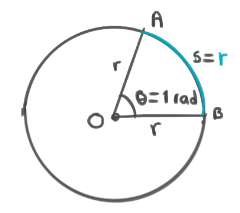
\includegraphics[width=4cm]{radian}
	\caption[Radian]{El radián.
		\begin{itemize}
			\item El arco $S$ tiene la misma medida que $\theta$ en grados
			\item El arco $S$ el unidades líneales mide $r$ (el radio).
		\end{itemize}
	}
	\labfig{radian}
\end{figure}

La unidad llamada radián se identifica a través del símbolo \textit{rad}

De la definición anterior debemos recordar siempre dos cosas:
\begin{itemize}
	\item \textbf{1 rad}\sidenote{Se lee como: ``un radián''} equivale a 
	$57.29^\circ$ \sidenote{No es necesario aprenderse este valor ya que para 
	calcularlo basta con recordar que el perímetro de la circunferencia es 
	$\boldsymbol{2r\pi}$. Y posteriormente realizar una sencilla regla de tres.}
	\item \fbox{ $\boldsymbol{\pi}$ \textbf{rad} equivale a $180^\circ$ }
\end{itemize}

\subsubsection{Conversión de grados a radianes y viceversa}
Los radianes y los grados tiene su equivalencia. De este modo, es posible medir 
los ángulos en grados o radianes según nos convenga. Para ello basta con un 
sencilla regla de tres, como se muestra a continuación.

\begin{example}
	Si queremos convertir $45^\circ$ a radianes.
	\begin{equation*}
	\begin{split}
		180^\circ &= \pi\; rad \\
		45^\circ &=  \boldsymbol{x}\\
		\Rightarrow x &= \dfrac{(45^\circ) (\pi\; rad)}{180^\circ}\\
		\therefore \boxed{ x = \dfrac{\pi}{4}\; rad }
	\end{split}
\end{equation*}
\end{example}

También se puede utilizar la regla de tres para convertir de radianes a grados.

\begin{example}
Convertir $\dfrac{\pi}{9}\; rad$ a grados.
\begin{equation*}
	\begin{split}
		180^\circ &= \pi\; rad \\
		\boldsymbol{x} &= \dfrac{\pi}{9}\; rad \\
		\Rightarrow x &= \dfrac{(180^\circ)
			\left(\dfrac{\pi}{9}\; rad \right)}{\pi\; rad} \\
		\therefore \boxed{ x = 20^\circ }
	\end{split}
\end{equation*}
\end{example}

Los dos tipos de conversiones se pueden realizar por medio de factores de 
conversión. Para ello tenemos las siguientes expresiones:

\begin{center}
	\renewcommand{\arraystretch}{1.2}
	\setlength{\tabcolsep}{20pt} % separacion de columnas
	\begin{tabular}{|c c |}
		\hline
		& \\
		\textbf{Grados a radianes} & \textbf{Radianes a grados}  \\ 
		$\alpha ^\circ \rightarrow\; rad$ & $rad \rightarrow \alpha ^\circ$ \\
		multiplicar por $\pmb{\dfrac{\pi}{180^\circ}}$ & 
		multiplicar por $\pmb{\dfrac{180^\circ}{\pi}}$ \\[5mm]		
		& \\
		\hline
	\end{tabular}
\end{center}

\begin{example}
	Convertir $75^\circ$ a radianes.
	$$75^\circ\left(\dfrac{\pi}{180^\circ} \right) = 
	\left( \dfrac{75^\circ}{180^\circ} \right) \pi\; rad = 
	\boxed{\left( \dfrac{5}{12}\right)\pi\; rad } $$
\end{example}

\begin{example}
	Convertir $\dfrac{7}{20} \pi\ rad$ a grados.
	$$\dfrac{7}{20} \pi\ rad \left(\dfrac{180^\circ}{\pi} \right) = 
		\left( \dfrac{7}{20} \right)(180^\circ) (\cancel{\pi\; rad})
		\left(\cancel{\dfrac{1}{\pi}}\right) = 
		7 \left(\dfrac{180^\circ}{20}\right) = 
		7 (9^\circ) = \boxed{63^\circ}
	$$
\end{example}

\begin{figure*}[hb!]
	\begin{kaoexercises}
		Convertir los siguientes ángulos a radianes
		\begin{multicols*}{4}
			\begin{enumerate}
				\setlength\itemsep{4mm}
				\item $210^\circ$
				\item $300^\circ$
				\item $225^\circ$
				\item $450^\circ$
				\item $72^\circ$
				\item $100^\circ$
				\item $330^\circ$
				\item $120^\circ$
				\item $135^\circ$
				\item $135^\circ$
			\end{enumerate}
		\end{multicols*}
		Convertir los siguientes ángulos a grados sexagesimales
		\begin{multicols*}{4}
			\begin{enumerate}
				\setlength\itemsep{4mm}
				\item $\dfrac{2}{3}\pi$
				\item $\dfrac{11}{6}\pi$
				\item $\dfrac{3}{4}\pi$
				\item $\dfrac{4}{3}\pi$
				\item $7 \pi$
				\item $\dfrac{1}{9} \pi$
				\item $\dfrac{13}{5} \pi$
				\item $\dfrac{1}{12} \pi$
				\item $\dfrac{5}{12} \pi$
				\item $\dfrac{9}{6} \pi$
			\end{enumerate}
		\end{multicols*}		
	\end{kaoexercises}
\end{figure*}

% Pseudo referencias
% https://oscarfruto.wixsite.com/angulos/sistema-ciclico
% http://maralboran.org/wikipedia/index.php/
%		Sistema_sexagesimal_de_medida_%281%C2%BA_ESO%29
\newpage
\section{Rectas paralelas y perpendiculares}

El análisis de líneas rectas puede visto desde varias ramas de la matemática, 
en este caso lo veremos desde el lado de la geometría euclídeana. Sin embargo,
es necesario destacar que se puede analizar también desde la geometría 
analítica, por lo tanto es posible tener varias definiciones de un concepto, 
sin que estas sen contrapongan.

%TODO:- Introducir el concepto de semi recta

\subsection{Paralelismo}

\marginnote{Cuando dos o más figuras geométricas se cortan (es decir, tienen 
puntos en común) se dice que se \textbf{intersecan}}

\begin{definition}
  Los rectas son \textbf{paraleas} en un plano si nunca se \textbf{intersectan} 
  y siempre guardan la misma distancia una de otra.
  \begin{center}
    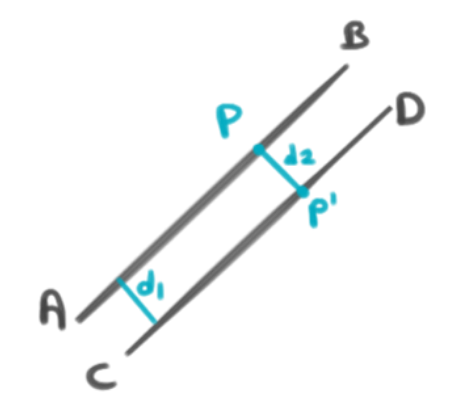
\includegraphics[width=4cm]{paralelas}
  \end{center}
  En la imagen podemos observar que $d_1 = d_ 2$, por lo tanto $\overline{AB}$ y 
  $\overline{CD}$ son paralelas.\\

  La condición de paralelismo se simboliza de matemática como:
  \[\overline{AB} \parallel \overline{CD}\]
  donde 
  \begin{itemize}
    \item [$\overline{AB}$] es el segmento AB
    \item [$\overline{CD}$] es el segmento CD
    \item [$\parallel$] es el simbolo de paralelismo
  \end{itemize}
\end{definition}

\subsubsection{El quinto postulado de Euclides}

El \textbf{quinto postulado de Euclides} estable que \textit{Data  
\textcolor{blue}{una recta} cualquiera, y \textcolor{orange}{un punto} 
fuera de ella, existe una y solo una recta paralela a la inicial, que pase 
por dicho punto}.

\subsection{Perpendicularidad}

\marginnote{El cuadrado en AOC indica un ángulo de $90^\circ$}

\begin{definition}
  Las rectas \textbf{perpendiculares} son aquellas que al intersectarse forman 
  un ángulo de $90^\circ$.
  \begin{center}
    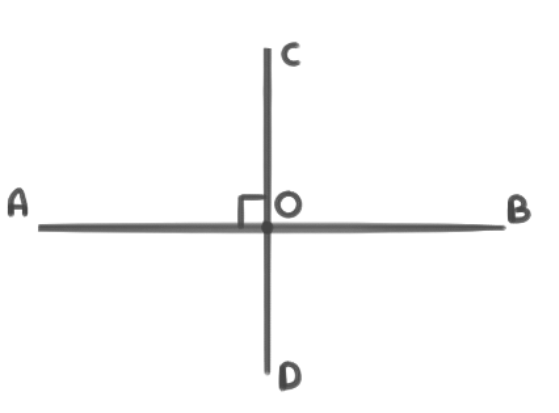
\includegraphics[width=4cm]{perpendicularidad}
  \end{center}
  La condición de perpendicularidad se simboliza de matemática como:
  \[\overline{AB} \perp \overline{CD}\]
  donde 
  \begin{itemize}
    \item [$\overline{AB}$] es el segmento AB
    \item [$\overline{CD}$] es el segmento CD
    \item [$\perp$] es el simbolo de perpendicularidad
  \end{itemize}

  En realidad, se forman 4 ángulos rectos ($90^\circ$), sin embargo, con que se 
  verifique la existencia de un ángulo recto basta.

\end{definition}

\subsubsection{Rectas oblicuas}

Por otra parte, si las rectas se intersecan en un ángulo \textbf{diferente} a 
$90^\circ$ se les conoce como \textbf{\textcolor{blue}{oblicuas}}

\subsection{Ángulos opuestos por el vértice}

Los ángulos opuestos por el vértice se forman con un par de rectas 
\sidenote{Algunos autores remarcan el hecho de que las rectas deber ser 
\textit{no paralelas}, sin embargo esto se puede obviar puesto que las rectas
deben tener un vértice en común.} tienen un vértice en común.

\begin{figure}[ht!]
	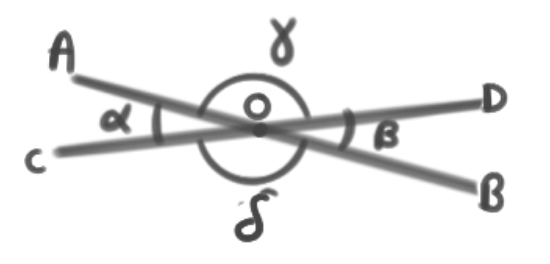
\includegraphics[width=7cm]{opporvertice}
	\caption[AngOpVertice]{Ángulos opuestos por el vértice.}
	\labfig{opporvertice}
\end{figure}

De la figura \reffig{opporvertice} se desprenden lo siguiente:
\begin{equation*}
\boxed{
\begin{array}{rcl}	
		\alpha &=& \beta \\
		\gamma &=& \delta 
	\end{array}
}
\end{equation*}

Las cuales se cumplen siempre para cualesquiera rectas con un vértice en común.

\textbf{¿Qué podrían preguntarnos en un examen? Veamos} \\

\textbf{NOTA:} Se recomienda tener nociones de aritmética y álgebra para revisar
los ejercicios propuestos.

\marginnote{\textbf{Recordatorio} \\ 
\begin{tabular}{c c}
  $\alpha + \beta = 90^\circ$ & 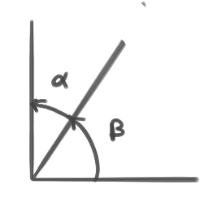
\includegraphics[width=1.5cm]{complementario} \\
	$\alpha + \beta = 180^\circ$ & 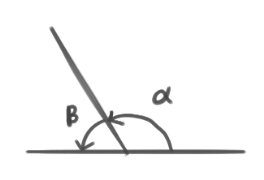
\includegraphics[width=2cm]{suplementario} \\ 
	$\alpha + \beta = 360^\circ$ & 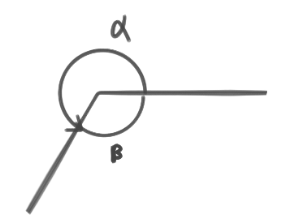
\includegraphics[width=2cm]{conjugado} 
\end{tabular}
}

\begin{example}
  Halla el valor de $x$ de la figura mostrada a continuación
  \begin{center}
    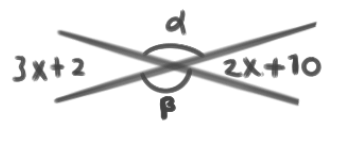
\includegraphics[width=5cm]{opvertEj01}
  \end{center}
  \textbf{Solución}. Por propiedades de ángulos opuesto por el vértice:
  \begin{equation*}
    \begin{array}{rcl}	
        3x + 2 & = & 2x + 10
    \end{array}
  \end{equation*}
  Y lo que resta es simplemente despejar $x$ por medio del álgebra
  \begin{align*}
      3x + 2 - 2x & = 10 \\
      3x - 2x & = 10 - 2 \\
      \Aboxed{x & = 8}
  \end{align*} 
  Eso quiere decir que el ángulo que mide $3x +2$ es igual a 
  \[3(8) + 2 = 26^\circ\]
\end{example}

\subsection{Ángulos adyacentes}

Se considera que dos ángulos son adyacentes si estos son contiguos 
(esta uno al lado del otro) y además, la suma de estos es igual a $180^\circ$.

\begin{figure}[ht!]
	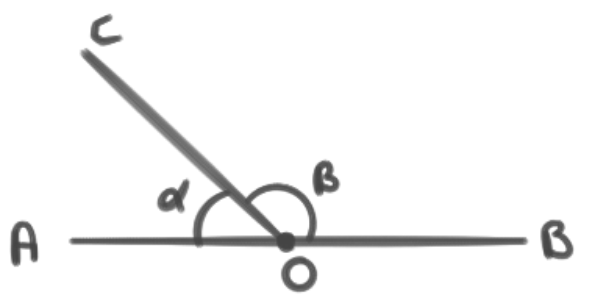
\includegraphics[width=6cm]{adyacente}
	\caption[AngAdyacentes]{Ángulos adyacentes.}
	\labfig{adyacente}
\end{figure}

De la figura \reffig{adyacente} se observa que 
\[\boxed{\alpha + \beta = 180^\circ}\]

\begin{example}
  Del ejemplo anterior, cuya figura se vuelve a mostar
  \begin{center}
    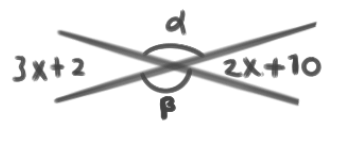
\includegraphics[width=5cm]{opvertEj01}
  \end{center}
  Hallar el valor de $\alpha$ y de $\beta$\\
  \textbf{Solución} 
  \[(3x +2) + \alpha = 180^\circ\]
  
  Ya conocemos el valor de $(3x +2)$ es igual a $26^\circ$ 
  \[\therefore (3x +2) + \alpha = 
    \textcolor{blue}{26^\circ} + \alpha = 180^\circ\]

  Despejando en valor de $\alpha$, se obtiene
  \begin{align*}
    \alpha & = 180^\circ - 26^\circ \\
    \therefore\; \Aboxed{\alpha & = 154^\circ } \\
  \end{align*}

\end{example}

\subsection{Rectas paralelas cortadas por una secante}

Los conceptos que veremos a continuación (ángulos interntos, externo y alternos)
nacen a partir del  análisis de \underline{dos rectas paralelas y otra oblicua},
que las corta y se conoce cómo \textit{secante}.

\begin{figure}[ht!]
	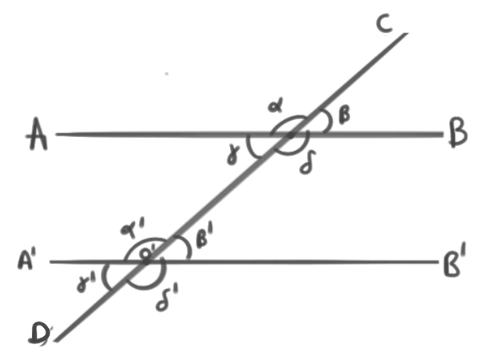
\includegraphics[width=9cm]{rectparalysec}
	\caption[RectasParalelas]{Rectas paralelas cortadas por una secante.
    \begin{itemize}
      \item $\overline{AB} \parallel \overline{A'B'}$
      \item $\overline{CD}$ es la recta \textit{secante}
    \end{itemize}
  }
	\labfig{rectparalysec}
\end{figure}

Como se observa en la figura \reffig{rectparalysec}, se producen \textit{dos} 
puntos de intersección, llamados $O$ y $O'$, producto de la recta secante con 
las paralelas.
\begin{itemize}
  \item Se generan \textit{4 ángulos} por cada intersección.
  \item Es decir, en total tenemos \textit{8 ángulos}.
\end{itemize}

Para identificar cada ángulo los nombraremos con base en lo siguiente:\\

\textbf{De acuerdo a su posición}

\begin{itemize}
  \item \textbf{Internos.} Son ángulos que están entre (o dentro) de las dos
    rectas paralelas.\\
    En la figura son: $\pmb{\gamma}$, $\pmb{\delta}$, 
    $\pmb{\alpha}'$, $\pmb{\beta}'$
  \item \textbf{Externos.} Son aquellos que están fuera de entre las dos rectas,
    es decir, están en la parte del plano que no esta comprendida entre las 
    rectas.\\
    En la figura son: $\pmb{\alpha}$, $\pmb{\beta}$, $\pmb{\gamma'}$, 
    $\pmb{\delta'}$
\end{itemize}

\textbf{De acuerdo a su referencia: con respecto a otro ángulo 
  y a la recta secante
}

Los ángulos que se mencionan a continuación se dan en pares y los varios son 
siempre los mismos. Por ejemplo en el caso de los anternos 
$\pmb{\alpha}$ = $\pmb{\delta'}$

\begin{itemize}
  \item \textbf{Alternos.} Dos ángulos son alternos si están en 
    \textit{lados opuestos} de la recta secante. Además ambos son 
    \textit{externos} o \textit{internos}.\\
    % y no comparten niguno de su lados. \\
    En la figura son:
    \begin{itemize}
      \item $\pmb{\alpha}$ y $\pmb{\delta'}$
      \item $\pmb{\beta}$ y $\pmb{\gamma'}$
      \item $\pmb{\gamma}$ y $\pmb{\beta'}$
      \item $\pmb{\delta}$ y $\pmb{\alpha'}$
    \end{itemize}
  \item \textbf{Conjugados.} Dos ángulos son correspondientes si están en el 
    \textit{mismo lado} de la recta secante y ambos son \textit{externos} o
    \textit{internos}.\\
    En la figura son:
    \begin{itemize}
      \item Para el lado izquierdo:
      \begin{itemize}
        \item $\pmb{\alpha}$ y $\pmb{\gamma}$
        \item $\pmb{\alpha'}$ y $\pmb{\gamma'}$
      \end{itemize}
      \item Para el lado derecho:
      \begin{itemize}
        \item $\pmb{\beta}$ y $\pmb{\delta}$
        \item $\pmb{\beta'}$ y $\pmb{\delta'}$
      \end{itemize}
    \end{itemize}
  \item \textbf{Correpondientes.} Dos ángulos son correspondientes si están del
    \textit{mismo lado} de la secante, uno es \textit{externo} y otro 
    \textit{interno}.\\
    % y no comparten ninguno de sus lados.\\
    En la figura son: 
    \begin{itemize}
      \item $\pmb{\alpha}$ y $\pmb{\alpha'}$
      \item $\pmb{\beta}$ y $\pmb{\beta'}$
      \item $\pmb{\gamma}$ y $\pmb{\gamma'}$
      \item $\pmb{\delta}$ y $\pmb{\delta'}$
    \end{itemize}
\end{itemize}

\textbf{De acuerdo a su posición y a su referencia}

\begin{marginfigure}[-6cm]
	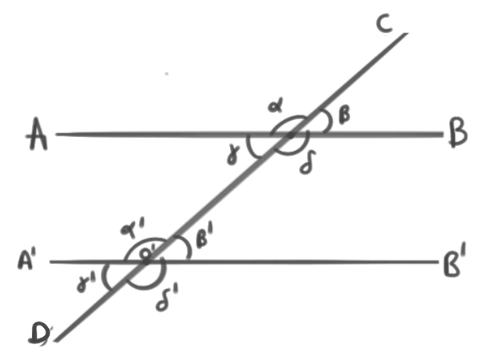
\includegraphics{rectparalysec}
	\caption[rectparalysec]{Rectas paralelas cortadas por una secante. En resumen
	  \begin{itemize}
      \item Ángulos alternos internos:
      \begin{itemize}
        \item $\pmb{\gamma} = \pmb{\beta'}$
        \item $\pmb{\delta} = \pmb{\alpha'}$
      \end{itemize}
      \item Ángulos alternos externos:
      \begin{itemize}
        \item $\pmb{\alpha} = \pmb{\delta'}$
        \item $\pmb{\beta} = \pmb{\gamma'}$
      \end{itemize}
      \item Ángulos correspondientes:
      \begin{itemize}
        \item $\pmb{\alpha} = \pmb{\alpha'}$
        \item $\pmb{\beta} = \pmb{\beta'}$
        \item $\pmb{\gamma} = \pmb{\gamma'}$
        \item $\pmb{\delta} = \pmb{\delta'}$
      \end{itemize}
    \end{itemize}
  }
	\labfig{pythagoras}
\end{marginfigure}

A la hora de habla de rectas cortadas por una secante \textit{lo más común} es 
referirse a los ángulos por su posición y su referencia.
Los siguiente ángulos se nombrar con base en us posición y referencia, como en 
el caso anterior, vienen el pares y su valor es el mismo:

\begin{itemize}
  \item \textbf{Ángulos alternos internos}. Son aquellos ángulos internos y que 
    a la vez son alternos.\\
    En la figura son: 
    \begin{itemize}
      \item $\pmb{\gamma}$ y $\pmb{\beta'}$
      \item $\pmb{\delta}$ y $\pmb{\alpha'}$
    \end{itemize}
    
  \item \textbf{Ángulos alternos externos}. Son ángulos que son externos y a la 
  vez alternos.\\
  En la figura son:
  \begin{itemize}
    \item $\pmb{\alpha}$ y $\pmb{\delta'}$
    \item $\pmb{\beta}$ y $\pmb{\gamma'}$
  \end{itemize}

  \item \textbf{Ángulos colaterales internos}. La suma de dos ángulos internos 
    situados del mismo lado de la secante da $180^\circ$.\\
    En la figura: 
    \begin{itemize}
      \item $\pmb{\gamma} + \pmb{\alpha'} = 180^\circ$
      \item $\pmb{\delta} + \pmb{\beta'} = 180^\circ$
    \end{itemize}

  \item \textbf{Ángulos colaterales externos}. La suma de dos ángulos externos 
    situados del mismo lado de la secante da $180^\circ$.\\  
    En la figura: 
    \begin{itemize}
      \item $\pmb{\alpha} + \pmb{\gamma'} = 180^\circ$
      \item $\pmb{\beta} + \pmb{\delta'} = 180^\circ$
    \end{itemize}
\end{itemize}

\begin{example}
  Hallar el valor de $x$ y de los 8 ángulos de la figura 
  \begin{center}
    \begin{tikzpicture}[scale=0.6]
      \node (cp) at (60:1) {};
      \node (cp2) at (-1,0) {};
      \draw (-3,0) coordinate (a) node[left] {$A$} -- 
      (0,0) coordinate (o) -- 
      (3,0) coordinate (b) node[right] {$B$};
      \draw (60:2) coordinate (d) node[right]{$D$} -- 
        (60:-5) coordinate (c) node[right,below] {$C$};
      \pic["$\alpha$",draw=orange,->,angle eccentricity=1.5,angle radius=5mm] 
        {angle=b--o--cp};
      \pic["$2x-20^\circ$",draw=blue,->,angle eccentricity=1.5,angle radius=5mm] 
        {angle=cp--o--a};   
      \pic["$\gamma$",draw=orange,->,angle eccentricity=1.5,angle radius=5mm] 
        {angle=a--o--c};   
      \pic["$\delta$",draw=blue,->,angle eccentricity=1.5,angle radius=5mm] 
        {angle=c--o--b};        
      % Parte de abajo    
      \draw (-4,-3) coordinate (a2) node[left] {$A'$} -- 
      (-1.7,-3) coordinate (o2) -- 
      (2,-3) coordinate (b2) node[right] {$B'$};  
      \pic["$\alpha$'",draw=orange,->,angle eccentricity=1.6,angle radius=5mm] 
        {angle=b2--o2--d}; 
      \pic["$\beta$'",draw=blue,->,angle eccentricity=1.2,angle radius=5mm] 
        {angle=d--o2--a2};   
      \pic["$2x$",draw=orange,->,angle eccentricity=1.6,angle radius=5mm] 
        {angle=a2--o2--c};  
      \pic["$\delta$'",draw=blue,->,angle eccentricity=1.5,angle radius=5mm] 
        {angle=c--o2--b2};            
    \end{tikzpicture}
  \end{center}
\end{example}

\newpage % This is not right

\begin{figure*}[ht!]
  \begin{kaoexercises}
    Encontrar \textit{todos} los ángulos faltantes
    \begin{multicols*}{2}
      \begin{enumerate}
        % 1
        \item \textbf{}\\
        \input{materias/matematicas/trigonometria/actividades/act_05/01}

        % 2
        \item \textbf{}\\
        \input{materias/matematicas/trigonometria/actividades/act_05/02}

        % 3
        \item \textbf{}\\
        \input{materias/matematicas/trigonometria/actividades/act_05/03}

        % 4
        \item \textbf{}\\
        \input{materias/matematicas/trigonometria/actividades/act_05/04}           

        % 5
        \item \textbf{}\\
        \input{materias/matematicas/trigonometria/actividades/act_05/05}           
        \columnbreak%
        % 6
        \item \textbf{}\\
        \input{materias/matematicas/trigonometria/actividades/act_05/06}           

        % 7
        \item \textbf{}\\
        \input{materias/matematicas/trigonometria/actividades/act_05/07}           
      
        % 8
        \item \textbf{}\\
        \input{materias/matematicas/trigonometria/actividades/act_05/08}           

        % 9
        \item \textbf{}\\
        \input{materias/matematicas/trigonometria/actividades/act_05/09}              
        % 10
        \item \textbf{}\\
        \input{materias/matematicas/trigonometria/actividades/act_05/10}                        
      \end{enumerate}
    \end{multicols*}
  \end{kaoexercises}
\end{figure*}

%TODO:- Historia de Eratóstenes

% PSEUDO BIBLIOGRAFIA
% https://edu.gcfglobal.org/es/geometria-basica/posicion-relativa-de-rectas/1/
% https://edu.gcfglobal.org/es/geometria-basica/
%   rectas-paralelas-cortadas-por-una-secante/1/
\newpage
\section{Triángulos}

\marginnote{Ahora sí empezaremos de lleno con el objeto de estudio de la 
trigonometría: los \textbf{triángulos}.}

\marginnote[2cm]{Como se vio en (REF) un triángulo en una figura plana de tres 
lados. Dichos lados en realidad son 3 semirectas que se intersectan una con otra 
en puntos llamados \textit{vértices}.}

\subsection{Clasificación de triángulos}

Es importante sbaer como se clasifican los triángulos ya que la mayoría de la 
bibliografía o concepto se aplica solo para cierto tipo de triángulos.\\

Los triángulos se clasifican por:
\begin{itemize}
  \item La \textit{longitud} de sus \textbf{lados}.
  \item La \textit{magnitud} de sus \textbf{ángulos}.
\end{itemize}
\subsubsection{Por sus lados}

\begin{figure*}[h!]
\def\arraystretch{1.5}%  1 is the default, change whatever you need
\caption[Clasificación de t2]{Clasificación de triángulos. 
	Se toma como base la magnitud de sus ángulos.
}
%TODO:- Corregir referencia de la tabla.
\labtab{clasiftriang2}\label{clasiftriang2}
\begin{tabular}{c  c  c }
	% \hline
  % TODO:- Corregir figuras
	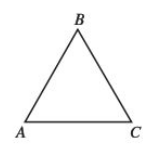
\includegraphics[width=4cm]{tequilatero} & 
	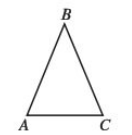
\includegraphics[width=4cm]{tisoceles}  & 
	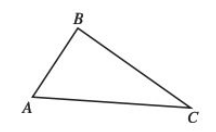
\includegraphics[width=4cm]{tescaleno} 
	\\ %\hline

	\textbf{Triángulo equilátero} & 
	\textbf{Triángulo isóceles} & 
	\textbf{Triángulo escaleno}                       
	\\ %\hline

	$\overline{AB} = \overline{AC} = \overline{BC}$ &
	$\overline{AB} = \overline{BC}$ &
	$\overline{AB} \ne \overline{AC} \ne \overline{BC}$ 
	\\

	\parbox{4cm}{
		\begin{center}
			Todos sus lados son iguales
		\end{center} 
	} & 
	\parbox{4cm}{
		\begin{center}
			Tiene 2 lados iguales
		\end{center} 
	} & 
	\parbox{4cm}{
		\begin{center}
			Todos sus lados son diferentes
		\end{center} 
	}                                 
\end{tabular}
% \end{adjustbox}
\end{figure*}

\subsubsection{Por sus ángulos}

\begin{figure*}[h!]
\def\arraystretch{1.5}%  1 is the default, change whatever you need
\caption[Clasificación de t]{Clasificación de triángulos. 
	Se toma como base la longitud de sus lados.
}
%TODO:- Corregir referencia de la tabla.
\labtab{clasiftriang}\label{clasiftriang}
\begin{tabular}{c  c  c }
	% \hline
  % TODO:- Corregir figuras
	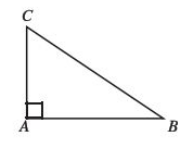
\includegraphics[width=4cm]{trectangulo} & 
	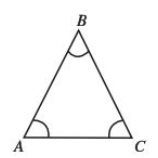
\includegraphics[width=4cm]{tacutangulo}  & 
	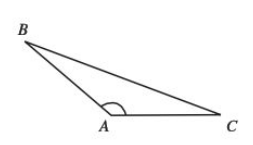
\includegraphics[width=4cm]{tobtusangulo} 
	\\ %\hline

	\textbf{Triángulo rectángulo} & 
	\textbf{Triángulo acutángulo} & 
	\textbf{Triángulo obtusángulo}                       
	\\ %\hline

	$\alpha = 90^\circ$ &
	$\alpha, \beta, \gamma < 90^\circ$ &
	$\alpha > 90^\circ$ 
	\\

	\parbox{4cm}{
		\begin{center}
			Tiene un ángulo recto
		\end{center} 
	} & 
	\parbox{4cm}{
		\begin{center}
			Sus 3 ángulos son agudos
		\end{center} 
	} & 
	\parbox{4cm}{
		\begin{center}
			Tiene un ángulo obtuso
		\end{center} 
	}                                 
\end{tabular}
% \end{adjustbox}
\end{figure*}

\newpage
\subsection{Rectas y puntos notables}

% TODO:- Recta de Euler

\begin{figure*}[h!]
\def\arraystretch{1.5}%  1 is the default, change whatever you need
\caption[Puntos notables]{Puntos notables y rectas en un triángulo}
%TODO:- Corregir referencia de la tabla.
\labtab{puntosnot}\label{puntosnot}
\begin{tabular}{c  c  c  c }
	\textbf{Altura} & 
	\textbf{Mediana} & 
	\textbf{Bisectriz} &
	\textbf{Mediatriz}
	\\
	\parbox{4cm}{ \begin{flushleft}
		Recta \textit{perpendicular} que va de un \textbf{vértice}
		al \textbf{lado opuesto}.
	\end{flushleft}}  & 
	\parbox{4cm}{ \begin{flushleft}
		Recta que va \textbf{vértice} con el \textbf{punto medio} 
		del lado opuesto. 
	\end{flushleft}}  & 
	\parbox{4cm}{ \begin{flushleft}		
		Recta que \textit{divide} a la \textit{mitad} a uno de los 	ángulos internos
		del triángulo. 
	\end{flushleft}}  & 		
	\parbox{4cm}{ \begin{flushleft}		
		Rectatextit{perpendicular} que pasa por el \textbf{punto medio}.
	\end{flushleft}}  
	\\
	\textbf{Ortocentro} & 
	\textbf{Baricentro} & 
	\textbf{Incentro} &
	\textbf{Circuncentro}
	\\
	\parbox{4cm}{ \begin{flushleft}
		Punto en donde se unen las \textbf{alturas}.
	\end{flushleft}}  & 
	\parbox{4cm}{ \begin{flushleft}
		Punto donde se intersectan las \textbf{medianas}.
	\end{flushleft}}  & 
	\parbox{4cm}{ \begin{flushleft}		
		Punto donde se intersectan las \textbf{bisectrices}.
	\end{flushleft}}  & 		
	\parbox{4cm}{ \begin{flushleft}		
		Punto donde se intersecan las \textbf{mediatrices}.
	\end{flushleft}}  
	\\
  % TODO:- Corregir figuras
	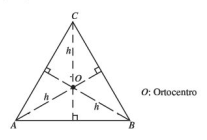
\includegraphics[width=4cm]{ortocentro} & 
	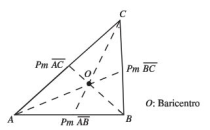
\includegraphics[width=4cm]{baricentro}  & 
	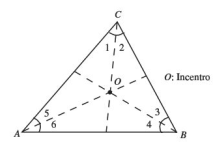
\includegraphics[width=4cm]{incentro} &
	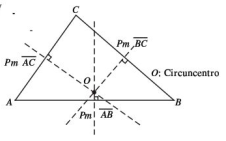
\includegraphics[width=4cm]{circuncentro} 
                                
\end{tabular}
% \end{adjustbox}
\end{figure*}

\subsection{Congruencia de triángulos}

2 triángulos son \textbf{congruentes}:
\marginnote{En pocas palabras, deben tener la misma forma y tamaño}
\begin{enumerate}[label=\alph*)]
	\item Sus \textit{lados} homólogos son iguales.
	\item Sus \textit{ángulos} homólogos son iguales.
\end{enumerate}

\marginnote{La notación para indicar congruencia es: $\cong$}

El concepto es muy sencillo, lo cierto es que en ``la vida real'' nunca nos
van a dar todas las medidas de un triángulo para poder comprobar que sus lados
y ángulos son homólogos, ¿Qué hacemos?\\

\textbf{\large3 casos}

\begin{figure*}[h!]
\def\arraystretch{1.5}%  1 is the default, change whatever you need
\caption[congruencia]{Casos de congruencia de triángulos. }
%TODO:- Corregir referencia de la tabla.
\labtab{congruencia}\label{congruencia}
\begin{tabular}{c  c  c }
	\textbf{Caso I} & 
	\textbf{Caso II} & 
	\textbf{Caso III}                       
	\\
	\textbf{Lados - Lado - Lado} & 
	\textbf{Ángulo - Lado - Ángulo} & 
	\textbf{Lado - Ángulo - Lado}                       
	\\
	$\begin{array} {lcl} 
		\overline{DE} & = & \overline{D'E'} \\ 
		\overline{EF} & = & \overline{E'F'} \\
		\overline{DF} & = & \overline{D'F'} 
	\end{array}$ &
	$\begin{array} {lcl} 
		H & = & H' \\ 
		\overline{HJ} & = & \overline{H'J'} \\
		J & = & J' 
	\end{array}$ &
	$\begin{array} {lcl} 
		\overline{KL} & = & \overline{K'L'} \\ 
		L & = & L' \\ 
		\overline{LM} & = & \overline{L'M'} 
	\end{array}$
	\\
  % TODO:- Corregir figuras
	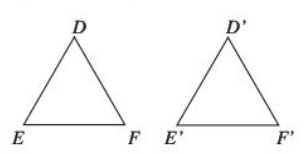
\includegraphics[width=4cm]{congruencia1} & 
	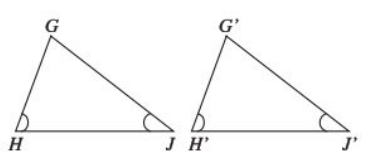
\includegraphics[width=4cm]{congruencia2}  & 
	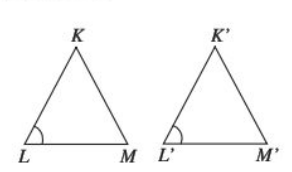
\includegraphics[width=4cm]{congruencia3} 
	
\end{tabular}
% \end{adjustbox}
\end{figure*}

\newpage
\subsection{Semejanza de triángulos}

2 triángulos son \textbf{semejantes} si:
\marginnote{Deben tener misma forma, pero diferente tamaño.}
\begin{enumerate}[label=\alph*)]
	\item Sus 3 \textit{ángulos} correspondientes son iguales.
	\item La \textit{proporción} de cada uno de sus 3 lados homólogos 
	\sidenote{Son aquellos cuyos águnos adyacentes son iguales} es proporcional.\\
		$$\dfrac{a}{a'} = \dfrac{b}{b'} = \dfrac{c}{c'}$$
\end{enumerate}

\textbf{\large3 casos}

\begin{figure*}[h!]
\def\arraystretch{1.5}%  1 is the default, change whatever you need
\caption[semejanza]{Casos de semejanza de triángulos. }
%TODO:- Corregir referencia de la tabla.
\labtab{semejanza}\label{semejanza}
\begin{tabular}{c  c  c }
	\textbf{Caso I} & 
	\textbf{Caso II} & 
	\textbf{Caso III}                       
	\\
	\textbf{2 ángulos homólogos} & 
	\textbf{3 Lados proporcionales} & 
	\parbox{5cm}{ \begin{center}
		\textbf{1 Ángulo igual y lados que forman dicho ángulos son proporcionales}                     
	\end{center}}  
	\\
	$\begin{array} {lcl} 
		C & = & C' \\ 
		A & = & A' 
	\end{array}$ &
	$\dfrac{a}{a'} = \dfrac{b}{b'} = \dfrac{c}{'c} $ &
	$\begin{array} {lcl} 
		K & = & K' \\ 
		\dfrac{g}{g'} &=& \dfrac{h}{h'}
	\end{array}$
	\\
  % TODO:- Corregir figuras
	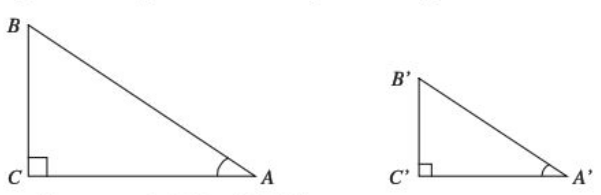
\includegraphics[width=5cm]{semejanza1} & 
	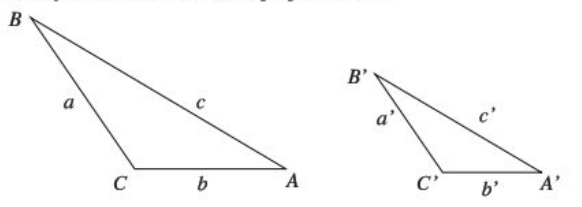
\includegraphics[width=5cm]{semejanza2}  & 
	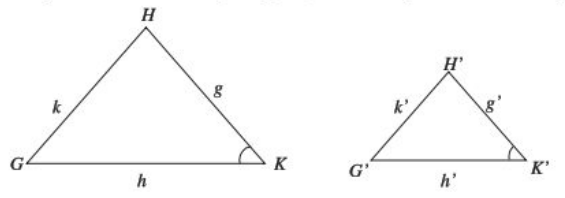
\includegraphics[width=5cm]{semejanza3} 
\end{tabular}
% \end{adjustbox}
\end{figure*}

% TODO:- Explicar proporciones.

\subsection{Teorema de Tales}

La consecuencia inmediata de la \textbf{semejanza del triángulos} es el
teorema conocido como \textbf{primer teorema de Tales}
\sidenote{A Tales de Mileto se le atribuyen dos teoremas con su nombre. 
El primero tiene que ver con la semejanza de triángulos y el segundo 
con triángulos inscritos en una circunferencia.}\\

El primer teorema de Tales dice que:\\

Si trazamos una recta paralela a uno de los lados de un triángulo se formará
otro que es semejante con el primero, como se observa en la figura 
\reffig{teorematales}.

\begin{figure}[ht!]
	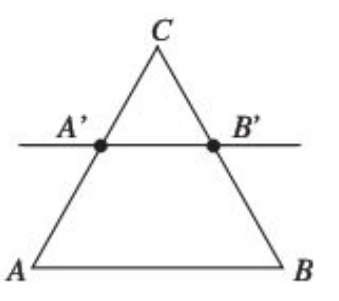
\includegraphics[width=5cm]{teorematales}
	\caption[teorematales]{Primer teorema de Tales.}
	\labfig{teorematales}
\end{figure}

Veamos un ejemplo:
% TODO:- Agregar ejemplo

% TODO:- Historia / Datos interesantes / Aplicaciones

\subsection{Teorema de Pitágoras}

El \textbf{teorema de Pitágoras} es uno de los teoremas que más aplicaciones 
tiene y del él han derivado muchos otros conceptos importantes de la 
trigonometría. 

\marginnote{A cada rato se emplea este concepto en física.}

El \textbf{teorema de Pitágoras} nos dice que:\\

Para cualquier \textit{triángulo rectángulo} el cuadrado de la hipotenusa
\sidenote{La hipotenusa es el lado más grande de un triángulo rectángulo.} es 
igual a la suma de los cuadrados de los catetos.\sidenote{Los catetos son los
lados que sobran después de definir quién es la hipotenusa.}

\begin{figure}[ht!]
	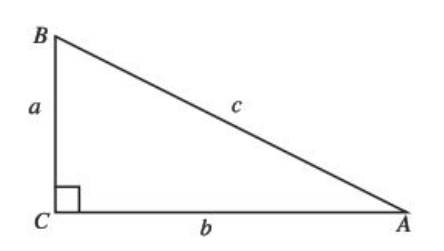
\includegraphics[width=5cm]{teoremapit}
	\caption[teoremapit]{Teorema de Pitágoras.}
	\labfig{teoremapit}
\end{figure}

En lenguaje matemático y con ayuda de la figura \reffig{teoremapit}, nos queda
como:

\[\boxed{c^2 = a^2 + b^2}\]

En donde: 
\begin{itemize}
	\item [\textbf{c}] es la \textit{hipotenusa} 
	\item [\textbf{a,b}] son los \textit{catetos}
\end{itemize}

Por medio del \textbf{teorema de Pitágoras} es posible clasificar o identificar
la naturalez de un triángulo, es decir, podemos decir si es \textit{acutángulo},
\textit{obtusángulo} o \textit{rectángulo}. 
\sidenote{Recuerda que el teorema de pitágoras se cumple (la igualdad) para 
triángulos rectángulos únicamente.}

\begin{enumerate}
	\item Si se cumple $c^2 = a^2 + b^2$, entonces hablamos de un triángulo 
		rectángulo.
	\item Si $c^2 \ne a^2 + b^2$ \sidenote[*]{Si la igualdad no se cumple}, 
		entonces puede que tengamos un triángulo \textit{acutángulo} o 
		\textit{obtusángulo}.
		\begin{itemize}
			\item Si $c^2 < a^2 + b^2$, entonce el triángulo es acutángulo.
			\item Si $c^2 > a^2 + b^2$, entonce el triángulo es obtusángulo.
		\end{itemize}
\end{enumerate}


\subsubsection{La semejanza en el triángulo rectángulo}

Dado un triángulo \textit{rectángulo}, a partir de la \textbf{hipotenusa} 
trazamos una \textbf{altura} hacia el vértice opuesto se formarán tres 
triángulos como muestra en la figura \reffig{semejrect}.

\begin{figure}[ht!]
	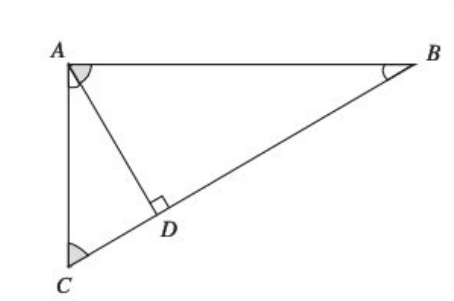
\includegraphics[width=5cm]{semejrect}
	\caption[semejrect]{Semejanza para triángulos rectángulos.}
	\labfig{semejrect}
\end{figure}

Los triángulos que se forman son semejantes de la siguiente manera

\begin{equation*}
\begin{array}{lcl}
	\widetriangle{ACD} & \sim & \widetriangle{BAD} \\
	\widetriangle{CAB} & \sim & \widetriangle{CDA} \\
	\widetriangle{CAB} & \sim & \widetriangle{ABD}
\end{array}
\end{equation*}

De lo anterior, puede demostrarse dos propiedades:

\begin{itemize}
	\setlength\itemsep{1.5em}
	\item $h^2 = \overline{CD}\cdot \overline{DB}$
	\item 
		$\begin{array}{lcl}
		\overline{AC} & = & \overline{CD} \cdot \overline{CB} \\
		\overline{AB} & = & \overline{CB} \cdot \overline{DB}
		\end{array}$
\end{itemize}


\subsection{Los ángulos (interiores) de un triángulo}

A continuación veremos las propiedades más importantes de los 
ángulos de un triángulo.

\begin{figure*}[h!]
\def\arraystretch{1.5}%  1 is the default, change whatever you need
\caption[propsTriangulos]{Propiedades elementales de los ángulos de los
	triángulos. 
}
%TODO:- Corregir referencia de la tabla.
\labtab{propstrig}\label{propstrig}
\begin{tabular}{c  c  c }
	\textbf{Propiedad I} & 
	\textbf{Propiedad II} & 
	\textbf{Propiedad III}                       
	\\
	\parbox{5cm}{ \begin{center}
		La suma de los ángulos interiores de un triángulo es igual a $180^\circ$	
	\end{center}}  &
	\parbox{5cm}{ \begin{center}
		La suma de los ángulos exteriores de un triángulo es igual a $360^\circ$
	\end{center}}  &
	\parbox{5cm}{ \begin{center}
		Un ángulo exterior es igual a la suma de los 2 interiores no adyacentes 
		a él
	\end{center}}  
	\\
  % TODO:- Corregir figuras
	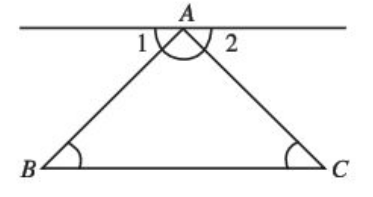
\includegraphics[width=5cm]{prop1} & 
	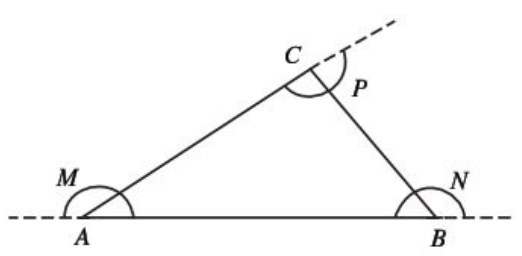
\includegraphics[width=5cm]{prop2}  & 
	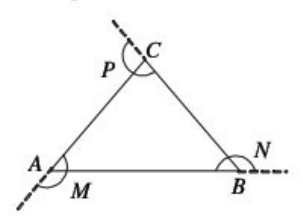
\includegraphics[width=5cm]{prop3} 
	\\ 
	$A + B + C = 180^\circ$ &
	$M + N + P = 360^\circ$&
	$\begin{array} {lcl} 
		M & = & B + C \\ 
		P & = & A + B \\ 
		N & = & A + C
	\end{array}$	
\end{tabular}
% \end{adjustbox}
\end{figure*}

\subsection{Razones trigonométricas}

Las razones trigonométricas son simplemente comparaciones de dos lados 
de un triángulo con respecto de un ángulo.

Primero, entendamos la terminología para nombrar cada uno de los lados de un 
triángulo.

% Insertar figura

\begin{itemize}
	\item \textbf{La hipotenusa} siempre es el lado más grande de un triángulo.
	\item \textbf{El cateto opuesto} se denomina así por que es el lado que está 
		en frente del ángulo de interés.
	\item \textbf{El cateto adyacente}, es el lado que está \textit{a un lado}
		del ángulo de interés.
\end{itemize}


% \graphicspath{{materias/matematicas/geoanalit/assets/}}

\setchapterimage[5.5cm]{bg03}
%https://www.123rf.com/stock-photo/trigonometry.html?sti=mwt5gbafw3l7clx5s6|
%&mediapopup=49203529
\chapter{Geometría Analítica}
\labch{geoanalit}
\section{Introducción}
\blindtext


% \graphicspath{{materias/matematicas/calcdif/assets/}}

\setchapterimage[6.5cm]{seaside}
\chapter[Cálculo diferencial]{Cálculo diferencial\footnotemark[0]}

\footnotetext{The credits for the image above the chapter title go to:
	Bushra Feroz --- Own work, CC~BY-SA~4.0, 
	\url{https://commons.wikimedia.org/w/index.php?curid=68724647}}

\section{Límites}

Figures and tables can be inserted just like in any standard 
\LaTeX\xspace document. The \Package{graphicx} package is already loaded 
and configured in such a way that the figure width is equal to the 
textwidth and the height is adjusted in order to maintain the original 
aspect ratio. As you may have imagined, the captions will be 
positioned\ldots well, in the margins. This is achieved with the help of 
the \Package{floatrow} package.

Here is a picture of Mona Lisa (\reffig{normalmonalisa}), as an example. 
The captions are formatted as the margin- and the side-notes; If you 
want to change something about captions you can use the command 
\Command{captsetup} from the \Package{caption} package. Remember that if 
you want to reference a figure, the label must come \emph{after} the 
caption!

\begin{figure}[hb]
	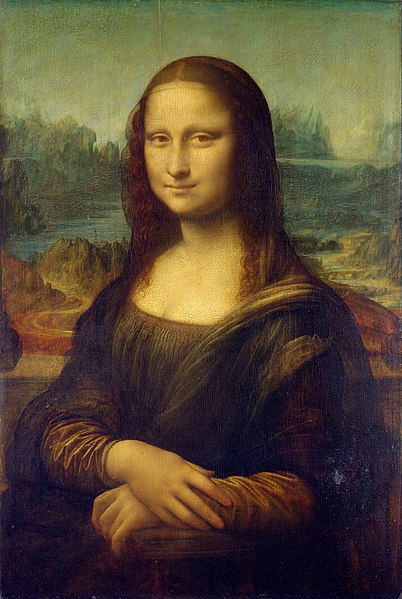
\includegraphics[width=0.45\textwidth]{monalisa}
	\caption[Mona Lisa, again]{It's Mona Lisa again. \blindtext}
	\labfig{normalmonalisa}
\end{figure}

While the format of the caption is managed by \Package{caption}, its 
position is handled by the \Package{floatrow} package. Achieving this 
result has been quite hard, but now I am pretty satisfied. In two-side 
mode, the captions are printed in the correct margin.

Tables can be inserted just as easily as figures, as exemplified by the 
following code:

\begin{lstlisting}[caption={Caption of a listing.}]
\begin{table}
\begin{tabular}{ c c c c }
	\toprule
	col1 & col2 & col3 & col 4 \\
	\midrule
	\multirow{3}{4em}{Multiple row} & cell2 & cell3 & cell4\\ &
	cell5 & cell6 & cell7 \\ &
	cell8 & cell9 & cell10 \\
	\multirow{3}{4em}{Multiple row} & cell2 & cell3 & cell4 \\ &
	cell5 & cell6 & cell7 \\ &
	cell8 & cell9 & cell10 \\
	\bottomrule
\end{tabular}
\end{table}
\end{lstlisting}

which results in the useless \vreftab{useless}.

\begin{table}[h]
\caption[A useless table]{A useless table.}
\labtab{useless}
\begin{tabular}{ c c c c }
	\toprule
	col1 & col2 & col3 & col 4 \\
	\midrule
	\multirow{3}{4em}{Multiple row} & cell2 & cell3 & cell4\\ &
	cell5 & cell6 & cell7 \\ &
	cell8 & cell9 & cell10 \\
	\multirow{3}{4em}{Multiple row} & cell2 & cell3 & cell4 \\ &
	cell5 & cell6 & cell7 \\ &
	cell8 & cell9 & cell10 \\
	\bottomrule
\end{tabular}
\end{table}

I don't have much else to say, so I will just insert some blind text. 
\blindtext

\section{Margin Figures and Tables}

Marginfigures can be inserted with the environment 
\Environment{marginfigure}. In this case, the whole picture is confined 
to the margin and the caption is below it. \reffig{marginmonalisa} is 
obtained with something like this:

\begin{lstlisting}[caption={Another caption.}]
\begin{marginfigure}
	\includegraphics{monalisa}
	\caption[The Mona Lisa]{The Mona Lisa.}
	\labfig{marginmonalisa}
\end{marginfigure}
\end{lstlisting}

There is also the \Environment{margintable} environment, of which 
\reftab{anotheruseless} is an example. Notice how you can place the 
caption above the table by just placing the \Command{caption} command 
before beginning the \Environment{tabular} environment. Usually, figure 
captions are below, while table captions are above. This rule is also 
respected for normal figures and tables: the captions are always on the 
side, but for figure they are aligned to the bottom, while for tables to 
the top.

\begin{margintable}
\caption[Another useless table]{Another useless table.}
\labtab{anotheruseless}
\raggedright
\begin{tabular}{ c c c c }
	\hline
	col1 & col2 & col3 \\
	\hline
	\multirow{3}{4em}{Multiple row} & cell2 & cell3 \\ & cell5 & cell6 
	\\ & cell8 & cell9 \\ \hline
\end{tabular}
\end{margintable}

Marginfigures and tables can be positioned with an optional offset 
command, like so:

\begin{lstlisting}
\begin{marginfigure}[offset]
	\includegraphics{seaside}
\end{marginfigure}
\end{lstlisting}

Offset ca be either a measure or a multiple of \Command{baselineskip}, 
much like with \Command{sidenote}, \Command{marginnote} and 
\Command{margintoc}.\todo{Improve this part.} If you are wondering how I 
inserted this orange bubble, have a look at the \Package{todo} package.

\section{Wide Figures and Tables}

\begin{figure*}[h!]
	\includegraphics{seaside}
	\caption[A wide seaside]{A wide seaside, and a wide caption.
		Credits: By Bushra Feroz --- Own work, CC BY-SA 4.0, 
		\url{https://commons.wikimedia.org/w/index.php?curid=68724647}}
\end{figure*}

With the environments \Environment{figure*} and \Environment{table*} you 
can insert figures which span the whole page width. The caption will be 
positioned below or above, according to taste.

You may have noticed the full width image at the very beginning of this 
chapter: that, however, is set up in an entirely different way, which 
you'll read about in \vrefch{layout}. Now it is time to tackle 
hyperreferences.

% \graphicspath{{materias/espanol/assets/}}

\pagelayout{wide} % No margins
\addpart{Español}
\pagelayout{margin} % Restore margins

\setchapterimage[5.5cm]{bg03}
%https://www.123rf.com/stock-photo/trigonometry.html?sti=mwt5gbafw3l7clx5s6|
%&mediapopup=49203529
\chapter{Español}
\labch{espanol}
\section{Introducción}
\blindtext


% \graphicspath{{materias/historiauniv/assets/}}

\pagelayout{wide} % No margins
\addpart{Historia Universal}
\pagelayout{margin} % Restore margins

\setchapterimage[5.5cm]{bg03}
%https://www.123rf.com/stock-photo/trigonometry.html?sti=mwt5gbafw3l7clx5s6|
%&mediapopup=49203529
\chapter{Historia Universal}
\labch{historiauniv}
\section{Introducción}
\blindtext


% \graphicspath{{materias/historiamx/assets/}}

\pagelayout{wide} % No margins
\addpart{Historia de México}
\pagelayout{margin} % Restore margins

\setchapterimage[5.5cm]{bg03}
%https://www.123rf.com/stock-photo/trigonometry.html?sti=mwt5gbafw3l7clx5s6|
%&mediapopup=49203529
\chapter{Historia de México}
\labch{historiamx}
\section{Introducción}
\blindtext


% \graphicspath{{materias/geografia/assets/}}

\pagelayout{wide} % No margins
\addpart{Geografía}
\pagelayout{margin} % Restore margins

\setchapterimage[5.5cm]{bg03}
%https://www.123rf.com/stock-photo/trigonometry.html?sti=mwt5gbafw3l7clx5s6|
%&mediapopup=49203529
\chapter{Geografía}
\labch{geografia}
\section{Introducción}
\blindtext


% \graphicspath{{materias/literatura/assets/}}

\pagelayout{wide} % No margins
\addpart{Literatura}
\pagelayout{margin} % Restore margins

\setchapterimage[5.5cm]{bg03}
%https://www.123rf.com/stock-photo/trigonometry.html?sti=mwt5gbafw3l7clx5s6|
%&mediapopup=49203529
\chapter{Literatura}
\labch{literatura}
\section{Introducción}
\blindtext


% \graphicspath{{materias/quimica/assets/}}

\pagelayout{wide} % No margins
\addpart{Química}
\pagelayout{margin} % Restore margins

\setchapterimage[5.5cm]{bg03}
%https://www.123rf.com/stock-photo/trigonometry.html?sti=mwt5gbafw3l7clx5s6|
%&mediapopup=49203529
\chapter{Química}
\labch{quimica}
\section{Introducción}
\blindtext

% \graphicspath{{materias/biologia/assets/}}

\pagelayout{wide} % No margins
\addpart{Biología}
\pagelayout{margin} % Restore margins

\setchapterimage[5.5cm]{bg03}
%https://www.123rf.com/stock-photo/trigonometry.html?sti=mwt5gbafw3l7clx5s6|
%&mediapopup=49203529
\chapter{Biología}
\labch{biologia}
\section{Introducción}
\blindtext

% \graphicspath{{materias/filosofia/assets/}}

\pagelayout{wide} % No margins
\addpart{Filosofía}
\pagelayout{margin} % Restore margins

\setchapterimage[5.5cm]{bg03}
%https://www.123rf.com/stock-photo/trigonometry.html?sti=mwt5gbafw3l7clx5s6|
%&mediapopup=49203529
\chapter{Filosofía}
\labch{filosofia}
\section{Introducción}
\blindtext



% \pagelayout{wide} % No margins
% \addpart{Class Options, Commands and Environments}
% \pagelayout{margin} % Restore margins

% \setchapterpreamble[u]{\margintoc}
\chapter{Class Options}
\labch{options}

In this chapter I will describe the most common options used, both the 
ones inherited from \Class{scrbook} and the \Class{kao}-specific ones. 
Options passed to the class modifies its default behaviour; beware 
though that some options may lead to unexpected results\ldots

\section{\Class{KOMA} Options}

The \Class{kaobook} class is based on \Class{scrbook}, therefore it 
understands all of the options you would normally pass to that class. If 
you have a lot of patience, you can read the \KOMAScript\xspace 
guide.\sidenote{The guide can be downloaded from 
\url{https://ctan.org/pkg/koma-script?lang=en}.} Actually, the reading 
of such guide is suggested as it is very instructive.

Every \KOMAScript\xspace option you pass to the class when you load it 
is automatically activated. In addition, in \Class{kaobook} some options 
have modified default values. For instance, the font size is 9.5pt and 
the paragraphs are separated by space,\sidenote[][-7mm]{To be precise, 
they are separated by half a line worth of space: the \Option{parskip} 
value is \enquote{half}.} not marked by indentation.

\section{\Class{kao} Options}

In the future I plan to add more options to set the paragraph formatting 
(justified or ragged) and the position of the margins (inner or outer in 
twoside mode, left or right in oneside mode).\sidenote{As of now, 
paragraphs are justified, formatted with \Command{singlespacing} (from 
the \Package{setspace} package) and \Command{frenchspacing}.}

I take this opportunity to renew the call for help: everyone is 
encouraged to add features or reimplement existing ones, and to send me 
the results. You can find the GitHub repository at 
\url{https://github.com/fmarotta/kaobook}.

\begin{kaobox}[frametitle=To Do]
Implement the \Option{justified} and \Option{margin} options. To be 
consistent with the \KOMAScript\xspace style, they should accept a 
simple switch as a parameter, where the simple switch should be 
\Option{true} or \Option{false}, or one of the other standard values for 
simple switches supported by \KOMAScript. See the \KOMAScript\xspace 
documentation for further information.
\end{kaobox}

The above box is an example of a \Environment{kaobox}, which will be 
discussed more thoroughly in \frefch{mathematics}. Throughout the book I 
shall use these boxes to remarks what still needs to be done.

\section{Other Things Worth Knowing}

A bunch of packages are already loaded in the class because they are 
needed for the implementation. These include:

\begin{itemize}
	\item etoolbox
	\item calc
	\item xifthen
	\item xkeyval
	\item xparse
	\item xstring
\end{itemize}

Many more packages are loaded, but they will be discussed in due time. 
Here, we will mention only one more set of packages, needed to change 
the paragraph formatting (recall that in the future there will be 
options to change this). In particular, the packages we load are:

\begin{itemize}
	\item ragged2e
	\item setspace
	\item hyphenat
	\item microtype
	\item needspace
	\item xspace
	\item xcolor (with options \Option{usenames,dvipsnames})
\end{itemize}

Some of the above packages do not concern paragraph formatting, but we 
nevertheless grouped them with the others. By default, the main text is 
justified and formatted with singlespacing and frenchspacing; the margin 
text is the same, except that the font is a bit smaller.

As a last warning, please be aware that the \Package{cleveref} package 
is not compatible with \Class{kaobook}. You should use the commands 
discussed in \refsec{hyprefs} instead.

\section{Document Structure}

We provide optional arguments to the \Command{title} and 
\Command{author} commands so that you can insert short, plain text 
versions of this fields, which can be used, typically in the half-title 
or somewhere else in the front matter, through the commands 
\Command{@plaintitle} and \Command{@plainauthor}, respectively. The PDF 
properties \Option{pdftitle} and \Option{pdfauthor} are automatically 
set by hyperref to the plain values if present, otherwise to the normal 
values.\sidenote[][*-1]{We think that this is an important point so 
we remark it here. If you compile the document with pdflatex, the PDF 
metadata will be altered so that they match the plain title and author 
you have specified; if you did not specify them, the metadata will be 
set to the normal title and author.}

There are defined two page layouts, \Option{margin} and \Option{wide}, 
and two page styles, \Option{plain} and \Option{fancy}. The layout 
basically concern the width of the margins, while the style refers to 
headers and footer; these issues will be 
discussed in \frefch{layout}.\sidenote[][6mm]{For now, suffice it to say that pages with 
the \Option{margin} layout have wide margins, while with the 
\Option{wide} layout the margins are absent. In \Option{plain} pages the 
headers and footer are suppressed, while in \Option{fancy} pages there 
is a header.} 

The commands \Command{frontmatter}, \Command{mainmatter}, and 
\Command{backmatter} have been redefined in order to automatically 
change page layout and style for these sections of the book. The front 
matter uses the \Option{margin} layout and the \Option{plain} page 
style. In the mainmatter the margins are wide and the headings are 
fancy. In the appendix the style and the layout do not change; however 
we use \Command{bookmarksetup\{startatroot\}} so that the bookmarks of 
the chapters are on the root level (without this, they would be under 
the preceding part). In the backmatter the margins shrink again and we 
also reset the bookmarks root.

% \setchapterpreamble[u]{\margintoc}
\chapter{Margin Stuff}

Sidenotes are a distinctive feature of all 1.5-column-layout books. 
Indeed, having wide margins means that some material can be displayed 
there. We use margins for all kind of stuff: sidenotes, marginnotes, 
small tables of contents, citations, and, why not?, special boxes and 
environments.

\section{Sidenotes}

Sidenotes are like footnotes, except that they go in the margin, where 
they are more readable. To insert a sidenote, just use the command 
\Command{sidenote\{Text of the note\}}. You can specify a 
mark\sidenote[O]{This sidenote has a special mark, a big O!} with \\ 
\Command{sidenote[mark]\{Text\}}, but you can also specify an offset, 
which moves the sidenote upwards or downwards, so that the full syntax is:

\begin{lstlisting}[style=kaolstplain]
\sidenote[mark][offset]{Text}
\end{lstlisting}

If you use an offset, you always have to add the brackets for the mark, 
but they can be empty.\sidenote{If you want to know more about the usage 
of the \Command{sidenote} command, read the documentation of the 
\Package{sidenotes} package.}

In \Class{kaobook} we copied a feature from the \Package{snotez} 
package: the possibility to specify a multiple of \Command{baselineskip} 
as an offset. For example, if you want to enter a sidenote with the 
normal mark and move it upwards one line, type:

\begin{lstlisting}[style=kaolstplain]
\sidenote[][*-1]{Text of the sidenote.}
\end{lstlisting}

As we said, sidenotes are handled through the \Package{sidenotes} 
package, which in turn relies on the \Package{marginnote} package.

\section{Marginnotes}

This command is very similar to the previous one. You can create a 
marginnote with \Command{marginnote[offset]\{Text\}}, where the offset 
argument can be left out, or it can be a multiple of 
\Command{baselineskip},\marginnote[-1cm]{While the command for margin 
notes comes from the \Package{marginnote} package, it has been redefined 
in order to change the position of the optional offset argument, which 
now precedes the text of the note, whereas in the original version it 
was at the end. We have also added the possibility to use a multiple of 
\Command{baselineskip} as offset. These things were made only to make 
everything more consistent, so that you have to remember less things!} 
\eg

\begin{lstlisting}[style=kaolstplain]
\marginnote[-12pt]{Text} or \marginnote[*-3]{Text}
\end{lstlisting}

\begin{kaobox}[frametitle=To Do]
A small thing that needs to be done is to renew the \Command{sidenote} 
command so that it takes only one optional argument, the offset. The 
special mark argument can go somewhere else. In other words, we want the 
syntax of \Command{sidenote} to resemble that of \Command{marginnote}.
\end{kaobox}

We load the packages \Package{marginnote}, \Package{marginfix} and 
\Package{placeins}. Since \Package{sidenotes} uses \Package{marginnote}, 
what we said for marginnotes is also valid for sidenotes. Side- and 
margin- notes are shifted slightly upwards 
(\Command{renewcommand\{\textbackslash marginnotevadjust\}\{3pt\}}) in 
order to allineate them to the bottom of the line of text where the note 
is issued.

\section{Footnotes}

Even though they are not displayed in the margin, we will discuss about 
footnotes here, since sidenotes are mainly intended to be a replacement 
of them. Footnotes force the reader to constantly move from one area of 
the page to the other. Arguably, marginnotes solve this issue, so you 
should not use footnotes. Nevertheless, for completeness, we have left 
the standard command \Command{footnote}, just in case you want to put a 
footnote once in a while.\footnote{And this is how they look like. 
Notice that in the PDF file there is a back reference to the text; 
pretty cool, uh?}

\section{Margintoc}

Since we are talking about margins, we introduce here the 
\Command{margintoc} command, which allows one to put small table of 
contents in the margin. Like other commands we have discussed, 
\Command{margintoc} accepts a parameter for the vertical offset, like 
so: \Command{margintoc[offset]}.

The command can be used in any point of the document, but we think it 
makes sense to use it just at the beginning of chapters or parts. In 
this document I make use of a \KOMAScript\xspace feature and put it in 
the chapter preamble, with the following code:

\marginnote{The font used in the margintoc is the same as the one for 
	the chapter entries in the main table of contents at the beginning 
	of the document.}

\begin{lstlisting}[style=kaolstplain]
\setchapterpreamble[u]{\margintoc}
\chapter{Chapter title}
\end{lstlisting}

\section{Marginlisting}

On some occasions it may happen that you have a very short piece of code 
that doesn't look good in the body of the text because it breaks the 
flow of narration: for that occasions, you can use a 
\Environment{marginlisting}. The support for this feature is still 
limited, especially for the captions, but you can try the following 
code:

\begin{marginlisting}[-1.35cm]
	\caption{An example of a margin listing.}
	\vspace{0.6cm}
	\begin{lstlisting}[language=Python,style=kaolstplain]
print("Hello World!")
	\end{lstlisting}
\end{marginlisting}

\begin{verbatim}
\begin{marginlisting}[-0.5cm]
	\caption{My caption}
	\vspace{0.2cm}
	\begin{lstlisting}[language=Python,style=kaolstplain]
	... code ...
	\end{lstlisting}
\end{marginlisting}
\end{verbatim}

Unfortunately, the space between the caption and the listing must be 
adjusted manually; if you find a better way, please let me know.

Not only textual stuff can be displayed in the margin, but also figures. 
Those will be the focus of the next chapter.

% \setchapterimage[6.5cm]{seaside}
\setchapterpreamble[u]{\margintoc}
\chapter[Figures and Tables]{Figures and Tables\footnotemark[0]}

\footnotetext{The credits for the image above the chapter title go to:
	Bushra Feroz --- Own work, CC~BY-SA~4.0, 
	\url{https://commons.wikimedia.org/w/index.php?curid=68724647}}

\section{Normal Figures and Tables}

Figures and tables can be inserted just like in any standard 
\LaTeX\xspace document. The \Package{graphicx} package is already loaded 
and configured in such a way that the figure width is equal to the 
textwidth and the height is adjusted in order to maintain the original 
aspect ratio. As you may have imagined, the captions will be 
positioned\ldots well, in the margins. This is achieved with the help of 
the \Package{floatrow} package.

Here is a picture of Mona Lisa (\reffig{normalmonalisa}), as an example. 
The captions are formatted as the margin- and the side-notes; If you 
want to change something about captions you can use the command 
\Command{captsetup} from the \Package{caption} package. Remember that if 
you want to reference a figure, the label must come \emph{after} the 
caption!

\begin{figure}[hb]
	\includegraphics[width=0.45\textwidth]{monalisa}
	\caption[Mona Lisa, again]{It's Mona Lisa again. \blindtext}
	\labfig{normalmonalisa}
\end{figure}

While the format of the caption is managed by \Package{caption}, its 
position is handled by the \Package{floatrow} package. Achieving this 
result has been quite hard, but now I am pretty satisfied. In two-side 
mode, the captions are printed in the correct margin.

Tables can be inserted just as easily as figures, as exemplified by the 
following code:

\begin{lstlisting}[caption={Caption of a listing.}]
\begin{table}
\begin{tabular}{ c c c c }
	\toprule
	col1 & col2 & col3 & col 4 \\
	\midrule
	\multirow{3}{4em}{Multiple row} & cell2 & cell3 & cell4\\ &
	cell5 & cell6 & cell7 \\ &
	cell8 & cell9 & cell10 \\
	\multirow{3}{4em}{Multiple row} & cell2 & cell3 & cell4 \\ &
	cell5 & cell6 & cell7 \\ &
	cell8 & cell9 & cell10 \\
	\bottomrule
\end{tabular}
\end{table}
\end{lstlisting}

which results in the useless \vreftab{useless}.

\begin{table}[h]
\caption[A useless table]{A useless table.}
\labtab{useless}
\begin{tabular}{ c c c c }
	\toprule
	col1 & col2 & col3 & col 4 \\
	\midrule
	\multirow{3}{4em}{Multiple row} & cell2 & cell3 & cell4\\ &
	cell5 & cell6 & cell7 \\ &
	cell8 & cell9 & cell10 \\
	\multirow{3}{4em}{Multiple row} & cell2 & cell3 & cell4 \\ &
	cell5 & cell6 & cell7 \\ &
	cell8 & cell9 & cell10 \\
	\bottomrule
\end{tabular}
\end{table}

I don't have much else to say, so I will just insert some blind text. 
\blindtext

\section{Margin Figures and Tables}

Marginfigures can be inserted with the environment 
\Environment{marginfigure}. In this case, the whole picture is confined 
to the margin and the caption is below it. \reffig{marginmonalisa} is 
obtained with something like this:

\begin{lstlisting}[caption={Another caption.}]
\begin{marginfigure}
	\includegraphics{monalisa}
	\caption[The Mona Lisa]{The Mona Lisa.}
	\labfig{marginmonalisa}
\end{marginfigure}
\end{lstlisting}

There is also the \Environment{margintable} environment, of which 
\reftab{anotheruseless} is an example. Notice how you can place the 
caption above the table by just placing the \Command{caption} command 
before beginning the \Environment{tabular} environment. Usually, figure 
captions are below, while table captions are above. This rule is also 
respected for normal figures and tables: the captions are always on the 
side, but for figure they are aligned to the bottom, while for tables to 
the top.

\begin{margintable}
\caption[Another useless table]{Another useless table.}
\labtab{anotheruseless}
\raggedright
\begin{tabular}{ c c c c }
	\hline
	col1 & col2 & col3 \\
	\hline
	\multirow{3}{4em}{Multiple row} & cell2 & cell3 \\ & cell5 & cell6 
	\\ & cell8 & cell9 \\ \hline
\end{tabular}
\end{margintable}

Marginfigures and tables can be positioned with an optional offset 
command, like so:

\begin{lstlisting}
\begin{marginfigure}[offset]
	\includegraphics{seaside}
\end{marginfigure}
\end{lstlisting}

Offset ca be either a measure or a multiple of \Command{baselineskip}, 
much like with \Command{sidenote}, \Command{marginnote} and 
\Command{margintoc}.\todo{Improve this part.} If you are wondering how I 
inserted this orange bubble, have a look at the \Package{todo} package.

\section{Wide Figures and Tables}

\begin{figure*}[h!]
	\includegraphics{seaside}
	\caption[A wide seaside]{A wide seaside, and a wide caption.
		Credits: By Bushra Feroz --- Own work, CC BY-SA 4.0, 
		\url{https://commons.wikimedia.org/w/index.php?curid=68724647}}
\end{figure*}

With the environments \Environment{figure*} and \Environment{table*} you 
can insert figures which span the whole page width. The caption will be 
positioned below or above, according to taste.

You may have noticed the full width image at the very beginning of this 
chapter: that, however, is set up in an entirely different way, which 
you'll read about in \vrefch{layout}. Now it is time to tackle 
hyperreferences.

% \setchapterstyle{kao}
%\setchapterpreamble[u]{\margintoc}
\chapter{References}
\labch{references}

\section{Citations}

\index{citations}
To cite someone \sidecite{Visscher2008,James2013} is very simple: just 
use the \Command{sidecite}\index{\Command{sidecite}} command. It does 
not have an offset argument yet, but it probably will in the future. 
This command supports multiple entries, as you can see, and by default 
it prints the reference on the margin as well as adding it to the 
bibliography at the end of the document. Note that the citations have 
nothing to do with the text,\sidecite{James2013} but they are completely 
random as they only serve the purpose to illustrate the feature.

For this setup I wrote a separate package, \Package{kaobiblio}, which 
you can find in the \Package{styles} directory and include in your main 
tex file. This package accepts all the options that you can pass to 
\Package{biblatex}, and actually it passes them to \Package{biblatex} 
under the hood. Moreover, it also defines some commands, like 
\Command{sidecite}, and environments that can be used within a 
\Class{kao} book.\sidenote{For this reason you should always use 
\Package{kaobiblio} instead of \Package{biblatex}, but the syntax and 
the options are exactly the same.}

As you have seen, the \Command{sidecite} command will print a citation 
in the margin. However, this command would be useless without a way to 
customise the format of the citation, so the \Class{kaobook} provides 
also the \Command{formatmargincitation} command. By \enquote{renewing} 
that command, you can choose which items will be printed in the margins. 
The best way to understand how it works is to see the actual definition 
of this command.

\begin{lstlisting}[style=kaolstplain,linewidth=1.5\textwidth]
\newcommand{\formatmargincitation}[1]{
	\parencite{#1}: \citeauthor*{#1} (\citeyear{#1}), \citetitle{#1}\\
}
\end{lstlisting}

Thus, the \Command{formatmargincitation} accepts one parameter, which is 
the citation key, and prints the parencite followed by a colon, then the 
author, then the year (in brackets), and finally the 
title.\sidecite{Battle2014} Now, suppose that you wish the margin 
citation to display the year and the author, followed by the title, and 
finally a fixed arbitrary string; you would add to your document:

\begin{lstlisting}[style=kaolstplain,linewidth=1.5\textwidth]
\renewcommand{\formatmargincitation}[1]{
	\citeyear{#1}, \citeauthor*{#1}: \citetitle{#1}; very interesting!\\
}
\end{lstlisting}

\renewcommand{\formatmargincitation}[1]{
	\citeyear{#1}, \citeauthor*{#1}: \citetitle{#1}; very interesting!\\
}

The above code results in citations that look like the 
following.\sidecite{Zou2005} Of course, changing the format is most 
useful when you also change the default bibliography style. For 
instance, if you want to use the \enquote{philosophy-modern} style for 
your bibliography, you might have something like this in the preamble:

\begin{lstlisting}[style=kaolstplain,linewidth=1.5\textwidth]
\usepackage[style=philosophy-modern]{styles/kaobiblio}
\renewcommand{\formatmargincitation}[1]{
	\sdcite{#1}\\
}
\addbibresource{main.bib}
\end{lstlisting}

\renewcommand{\formatmargincitation}[1]{
	\parencite{#1}: \citeauthor*{#1} (\citeyear{#1}), \citetitle{#1}\\
}

The commands like \Command{citeyear}, \Command{parencite} and 
\Command{sdcite} are just examples. A full reference of the available 
commands can be found in this 
\href{http://tug.ctan.org/info/biblatex-cheatsheet/biblatex-cheatsheet.pdf}{cheatsheet}, 
under the \enquote{Citations} section.

Finally, to compile a document containing citations, you need to use an 
external tool, which for this class is biber. You need to run the 
following (assuming that your tex file is called main.tex):

\begin{lstlisting}[style=kaolstplain]
$ pdflatex main
$ biber main
$ pdflatex main
\end{lstlisting}

\section{Glossaries and Indices}

\index{glossary}
The \Class{kaobook} class loads the packages \Package{glossaries} and 
\Package{imakeidx}, with which you can add glossaries and indices to 
your book. For instance, I previously defined some glossary entries and 
now I am going to use them, like this: \gls{computer}. 
\Package{glossaries} also allows you to use acronyms, like the 
following: this is the full version, \acrfull{fpsLabel}, and this is the 
short one \acrshort{fpsLabel}. These entries will appear in the glossary 
in the backmatter.

Unless you use \href{https://www.overleaf.com}{Overleaf} or some other 
fancy IDE for \LaTeX, you need to run an external command from your 
terminal in order to compile a document with a glossary. In particular, 
the commands required are:\sidenote{These are the commands you 
would run in a UNIX system; I have no idea on how it works in Windows.}

\begin{lstlisting}[style=kaolstplain]
$ pdflatex main
$ makeglossaries main
$ pdflatex main
\end{lstlisting}

Note that you need not run \texttt{makeglossaries} every time you 
compile your document, but only when you change the glossary entries.

\index{index}
To create an index, you need to insert the command 
\lstinline|\index{subject}| whenever you are talking about 
\enquote{subject} in the text. For instance, at the start of this 
paragraph I would write \lstinline|index{index}|, and an entry would be 
added to the Index in the backmatter. Check it out!

\marginnote[2mm]{In theory, you would need to run an external command 
for the index as well, but luckily the package we suggested, 
	\Package{imakeidx}, can compile the index automatically.}

\index{nomenclature}
A nomenclature is just a special kind of index; you can find one at the end of
this book. To insert a nomenclature, we use the package \Package{nomencl} and
add the terms with the command \Command{nomenclature}. We put then a
\Command{printnomenclature} where we want it to appear.

Also with this package we need to run an external command to compile the 
document, otherwise the nomenclature will not appear:

\begin{lstlisting}[style=kaolstplain]
$ pdflatex main
$ makeindex main.nlo -s nomencl.ist -o main.nls
$ pdflatex main
\end{lstlisting}

These packages are all loaded in 
\href{style/packages.sty}{packages.sty}, one of the files that come with 
this class. However, the configuration of the elements is best done in 
the main.tex file, since each book will have different entries and 
styles.

Note that the \Package{nomencl} package caused problems when the 
document was compiled, so, to make a long story short, I had to prevent 
\Package{scrhack} to load the hack-file for \Package{nomencl}. When 
compiling the document on Overleaf, however, this problem seem to 
vanish.

\marginnote[-19mm]{This brief section was by no means a complete 
reference on the subject, therefore you should consult the documentation 
of the above package to gain a full understanding of how they work.}

\section{Hyperreferences}
\labsec{hyprefs}

\index{hyperreferences}
In this class we provide a handy sub-package to help you referencing the 
same elements always in the same way, for consistency across the book. 
First, you can label each element with a specific command. For instance, 
should you want to label a chapter, you would put 
\lstinline|\labch{chapter-title}| right after the \Command{chapter} 
directive. This is just a convienence, because \Command{labch} is 
actually just an alias to \lstinline|\label{ch:chapter-title}|, so it 
spares you the writing of \enquote{ch}. We defined similar commands for 
many typically labeled elements, including:

\begin{multicols}{2}
\setlength{\columnseprule}{0pt}
\begin{itemize}
	\item Page: \Command{labpage}
	\item Part: \Command{labpart}
	\item Chapter: \Command{labch}
	\item Section: \Command{labsec}
	\item Figure: \Command{labfig}
	\item Table: \Command{labtab}
	\item Definition: \Command{labdef}
	\item Theorem: \Command{labthm}
	\item Proposition: \Command{labprop}
	\item Lemma: \Command{lablemma}
	\item Remark: \Command{labremark}
	\item Example: \Command{labexample}
	\item Exercise: \Command{labexercise}
\end{itemize}
\end{multicols}

Of course, we have similar commands for referencing those elements. 
However, since the style of the reference should depend on the context, 
we provide different commands to reference the same thing. For instance, 
in some occasions you may want to reference the chapter by name, but 
other times you want to reference it only by number. In general, there 
are four reference style, which we call plain, vario, name, and full. 

The plain style references only by number. It is accessed, for chapters, 
with \lstinline|\refch{chapter-title}| (for other elements, the syntax 
is analogous). Such a reference results in: \refch{references}.

The vario and name styles rest upon the \Package{varioref} package. 
Their syntax is \lstinline|\vrefch{chapter-title}| and 
\lstinline|\nrefch{chapter-title}|, and they result in: 
\vrefch{references}, for the vario style, and: \nrefch{references}, for 
the name style. As you can see, the page is referenced in 
\Package{varioref} style.

The full style references everything. You can use it with 
\lstinline|\frefch{chapter-title}| and it looks like this: 
\frefch{references}.

Of course, all the other elements have similar commands (\eg for parts 
you would use \lstinline|\vrefpart{part-title}| or something like that). 
However, not all elements implement all the four styles. The commands 
provided should be enough, but if you want to see what is available or 
to add the missing ones, have a look at the 
\href{styles/kaorefs.sty}{attached package}.


% \pagelayout{wide} % No margins
% \addpart{Design and Additional Features}
% \pagelayout{margin} % Restore margins

% \setchapterimage[6cm]{seaside}
\setchapterpreamble[u]{\margintoc}
\chapter{Page Design}
\labch{layout}

\section{Headings}

So far, in this document I used two different styles for the chapter 
headings: one has the chapter name, a rule and, in the margin, the 
chapter number; the other has an image at the top of the page, and the 
chapter title is printed in a box (like for this chapter). There is one 
additional style, which I used only in the appendix 
(\vrefpage{appendix}); there, the chapter title is enclosed in two 
horizontal rules, and the chapter number (or letter, in the case of the 
appendix) is above it.\sidenote{To be honest, I do not think that mixing 
heading styles like this is a wise choice, but in this document I did it 
only to show you how they look.}

Every book is unique, so it makes sense to have different styles from 
which to choose. Actually, it would be awesome if whenever a 
\Class{kao}-user designs a new heading style, he or she added it to the 
three styles already present, so that it will be available for new users 
and new books.

The choice of the style is made simple by the \Command{setchapterstyle} 
command. It accepts one option, the name of the style, which can be: 
\enquote{plain}, \enquote{kao}, or \enquote{lines}.\sidenote{Plain is 
the default \LaTeX\xspace title style; the other ones are self 
explanatory.} If instead you want the image style, you have to use the 
command \Command{setchapterimage}, which accepts the path to the image 
as argument; you can also provide an optional parameter in square 
brackets to specify the height of the image.

Let us make some examples. In this book, I begin a normal chapter with 
the lines:

\begin{lstlisting}
\setchapterstyle{kao}
\setchapterpreamble[u]{\margintoc}
\chapter{Title of the Chapter}
\labch{title}
\end{lstlisting}

In Line 1 I choose the style for the title to be \enquote{kao}. Then, I 
specify that I want the margin toc. The rest is ordinary administration 
in \LaTeX, except that I use my own \Command{labch} to label the 
chapter. Actually, the \Command{setchapterpreamble} is a standard 
\KOMAScript\xspace one, so I invide you to read about it in the KOMA 
documentation. Once the chapter style is set, it holds until you change 
it.\sidenote{The \Command{margintoc} has to be specified at every 
chapter. Perhaps in the future this may change; it all depends on how 
this feature will be welcomed by the users, so keep in touch with me if 
you have preferences!} Whenever I want to start a chapter with an image, 
I simply write:

\begin{lstlisting}
\setchapterimage[7cm]{path/to/image.png} % Optionally specify the height
\setchapterpreamble[u]{\margintoc}
\chapter{Catchy Title} % No need to set a chapter style
\labch{catchy}
\end{lstlisting}

If you prefer, you can also specify the style at the beginning of the 
main document, and that style will hold until you change it again.

\section{Headers \& Footers}

Headers and footers in \KOMAScript\xspace are handled by the 
\Package{scrlayer-scrpage} package. There are two basic style: 
\enquote{scrheadings} and \enquote{plain.scrheadings}. The former is 
used for normal pages, whereas the latter is used in title pages (those 
where a new chapter starts, for instance) and, at least in this book, in 
the front matter. At any rate, the style can be changed with the 
\Command{pagestyle} command, \eg 
\lstinline|\pagestyle{plain.scrheadings}|.

In both stles, the footer is completely empty. In plain.scrheadings, 
also the header is absent (otherwise it wouldn't be so plain\ldots), but 
in the normal style the design is reminescent of the \enquote{kao} style 
for chapter titles.

\begin{kaobox}[frametitle=To Do]
The \Option{twoside} class option is still unstable and may lead to 
unexpected behaviours. As always, any help will be greatly appreciated.
\end{kaobox}

\section{Table of Contents}

Another important part of a book is the table of contents. By default, 
in \Class{kaobook} there is an entry for everything: list of figures, 
list of tables, bibliographies, and even the table of contents itself. 
Not everybody might like this, so we will provide a description of the 
changes you need to do in order to enable or disable each of these 
entries. In the following \reftab{tocentries}, each item corresponds to 
a possible entry in the \acrshort{tocLabel}, and its description is the 
command you need to provide to have such entry. These commands are 
specified in the attached \href{style/style.sty}{style 
package},\sidenote{In the same file, you can also choose the titles of 
these entries.} so if you don't want the entries, just comment the 
corresponding lines.

Of course, some packages, like those for glossaries and indices, will 
try to add their own entries.\marginnote{In a later section, we will see 
how you can define your own floating environment, and endow it with an 
entry in the \acrshort{tocLabel}.} In such cases, you have to follow the 
instructions specific to that package. Here, since we have talked about 
glossaries and notations in \refch{references}, we will biefly see how 
to configure them.

\begin{table}
\footnotesize
\caption{Commands to add a particular entry to the table of contents.}
\labtab{tocentries}
\begin{tabular}{ l l }
	\toprule
	Entry & Command to Activate \\
	\midrule
	Table of Contents & \lstinline|\setuptoc{toc}{totoc}| \\
	List of Figs and Tabs & \lstinline|\PassOptionsToClass{toc=listof}{\@baseclass}| \\
	Bibliography & \lstinline|\PassOptionsToClass{toc=bibliography}{\@baseclass}| \\
	\bottomrule
\end{tabular}
\end{table}

For the \Package{glossaries} package, use the \enquote{toc} option when 
you load it: \lstinline|\usepackage[toc]{glossaries}|. For 
\Package{nomencl}, pass the \enquote{intoc} option at the moment of 
loading the package. Both \Package{glossaries} and \Package{nomencl} are 
loaded in the attached \href{style/packages.sty}{\enquote{packages} 
package}.

Additional configuration of the table of contents can be performed 
through the packages \Package{etoc}, which is loaded because it is 
needed for the margintocs, or the more traditional \Package{tocbase}. 
Read the respective documentations if you want to be able to change the 
default \acrshort{tocLabel} style.\sidenote[][*-1]{(And please, send me 
a copy of what you have done, I'm so curious!)}

\section{Page Layout}

Besides the page style, you can also change the width of the content of 
a page. This is particularly useful for pages dedicated to part titles, 
where having the 1.5-column layout might be a little awkward, or for 
pages where you only put figures, where it is important to exploit all 
the available space.

In practice, there are two layouts: \enquote{wide} and \enquote{margin}. 
The former suppresses the margins and allocates the full page for 
contents, while the latter is the layout used in most of the pages of 
this book, including this one. The wide layout is also used 
automatically in the front and back matters.

To change page layout, use the \Command{pagelayout} command. For 
example, when I start a new part, I write:

\begin{lstlisting}
\pagelayout{wide}
\addpart{Title of the New Part}
\pagelayout{margin}
\end{lstlisting}

\section{Numbers \& Counters}

In this short section we shall see how dispositions, sidenotes and 
figures are numbered in the \Class{kaobook} class.

By default, dispositions are numbered up to the section. This is 
achieved by setting: \lstinline|\setcounter{secnumdepth}{1}|.

The sidenotes counter is the same across all the document, but if you 
want it to reset at each chapter, just uncomment the line

\begin{lstlisting}[style=kaolstplain]
\counterwithin*{sidenote}{chapter}
\end{lstlisting}

in the \Package{styles/style.sty} package provided by this class.

Figure and Table numbering is also per-chapter; to change that, use 
something like:

\begin{lstlisting}[style=kaolstplain]
\renewcommand{\thefigure}{\arabic{section}.\arabic{figure}}
\end{lstlisting}

\section{White Space}

One of the things that I find most hard in \LaTeX\xspace is to finely 
tune the white space around objects. There are not fixed rules, each 
object needs its own adjustment. Here we shall see how some spaces are 
defined at the moment in this class.\marginnote{Attention! This section 
may be incomplete.}

\textbf{Space around figures and tables}

\begin{lstlisting}[style=kaolstplain]
\renewcommand\FBaskip{.4\topskip}
\renewcommand\FBbskip{\FBaskip}
\end{lstlisting}

\textbf{Space around captions}

\begin{lstlisting}[style=kaolstplain]
\captionsetup{
	aboveskip=6pt,
	belowskip=6pt
}
\end{lstlisting}

\textbf{Space around displays (\eg equations)}

\begin{lstlisting}[style=kaolstplain]
\setlength\abovedisplayskip{6pt plus 2pt minus 4pt}
\setlength\belowdisplayskip{6pt plus 2pt minus 4pt}
\abovedisplayskip 10\p@ \@plus2\p@ \@minus5\p@
\abovedisplayshortskip \z@ \@plus3\p@
\belowdisplayskip \abovedisplayskip
\belowdisplayshortskip 6\p@ \@plus3\p@ \@minus3\p@
\end{lstlisting}

% \setchapterstyle{kao}
\setchapterpreamble[u]{\margintoc}
\chapter{Mathematics and Boxes}
\labch{mathematics}

\section{Theorems}

Despite most people complain at the sight of a book full of equations, 
mathematics is an important part of many books. Here, we shall 
illustrate some of the possibilities. We believe that theorems, 
definitions, remarks and examples should be emphasised with a shaded 
background; however, the colour should not be to heavy on the eyes, so 
we have chosen a sort of light yellow.\sidenote{The boxes are all of the 
same colour here, because we did not want our document to look like 
\href{https://en.wikipedia.org/wiki/Harlequin}{Harlequin}.}

\begin{definition}
\labdef{openset}
Let $(X, d)$ be a metric space. A subset $U \subset X$ is an open set 
if, for any $x \in U$ there exists $r > 0$ such that $B(x, r) \subset 
U$. We call the topology associated to d the set $\tau\textsubscript{d}$ 
of all the open subsets of $(X, d).$
\end{definition}

\refdef{openset} is very important. I am not joking, but I have inserted 
this phrase only to show how to reference definitions. The following 
statement is repeated over and over in different environments.

\begin{theorem}
A finite intersection of open sets of (X, d) is an open set of (X, d), 
i.e $\tau\textsubscript{d}$ is closed under finite intersections. Any 
union of open sets of (X, d) is an open set of (X, d).
\end{theorem}

\begin{proposition}
A finite intersection of open sets of (X, d) is an open set of (X, d), 
i.e $\tau\textsubscript{d}$ is closed under finite intersections. Any 
union of open sets of (X, d) is an open set of (X, d).\marginnote{You can even insert footnotes inside the theorem 
	environments; they will be displayed at the bottom of the box.}
\end{proposition}

\begin{lemma}
A finite intersection\footnote{I'm a footnote} of open sets of (X, d) is 
an open set of (X, d), i.e $\tau\textsubscript{d}$ is closed under 
finite intersections. Any union of open sets of (X, d) is an open set of 
(X, d).
\end{lemma}

You can safely ignore the content of the theorems\ldots I assume that if 
you are interested in having theorems in your book, you already know 
something about the classical way to add them. These example should just 
showcase all the things you can do within this class.

\begin{corollary}[Finite Intersection, Countable Union]
A finite intersection of open sets of (X, d) is an open set of (X, d), 
i.e $\tau\textsubscript{d}$ is closed under finite intersections. Any 
union of open sets of (X, d) is an open set of (X, d).
\end{corollary}

\begin{proof}
The proof is left to the reader as a trivial exercise. Hint: \blindtext
\end{proof}

\begin{definition}
Let $(X, d)$ be a metric space. A subset $U \subset X$ is an open set 
if, for any $x \in U$ there exists $r > 0$ such that $B(x, r) \subset 
U$. We call the topology associated to d the set $\tau\textsubscript{d}$ 
of all the open subsets of $(X, d).$\marginnote{
	Here is a random equation, just because we can:
	\begin{equation*}
  x = a_0 + \cfrac{1}{a_1
          + \cfrac{1}{a_2
          + \cfrac{1}{a_3 + \cfrac{1}{a_4} } } }
	\end{equation*}
}
\end{definition}

\begin{example}
Let $(X, d)$ be a metric space. A subset $U \subset X$ is an open set 
if, for any $x \in U$ there exists $r > 0$ such that $B(x, r) \subset 
U$. We call the topology associated to d the set $\tau\textsubscript{d}$ 
of all the open subsets of $(X, d).$
\end{example}

\begin{remark}
Let $(X, d)$ be a metric space. A subset $U \subset X$ is an open set 
if, for any $x \in U$ there exists $r > 0$ such that $B(x, r) \subset 
U$. We call the topology associated to d the set $\tau\textsubscript{d}$ 
of all the open subsets of $(X, d).$
\end{remark}

As you may have noticed, definitions, example and remarks have 
independent counters; theorems, propositions, lemmas and corollaries 
share the same counter.

\begin{remark}
Here is how an integral looks like inline: $\int_{a}^{b} x^2 dx$, and 
here is the same integral displayed in its own paragraph:
\[\int_{a}^{b} x^2 dx\]
\end{remark}

We provide two files for the theorem styles: 
\href{style/plaintheorems.sty}{plaintheorems.sty}, which you should 
include if you do not want coloured boxes around theorems; and 
\href{style/mdftheorems.sty}{mdftheorems.sty}, which is the one used for 
this document.\sidenote{The plain one is not showed, but actually it is 
exactly the same as this one, only without the yellow boxes.} Of course, 
you will have to edit these files according to your taste and the 
general style of the book.

\section[Boxes \& Environments]{Boxes \& Custom Environments
\sidenote[][*1.8]{Notice that in the table of contents and in the 
	header, the name of this section is \enquote{Boxes \& Environments}; 
	we achieved this with the optional argument of the \texttt{section} 
	command.}}

Say you want to insert a special section, an optional content or just 
something you want to emphasise. We think that nothing works better than 
a box in these cases. We used \Package{mdframed} to construct the ones 
shown below. You can create and modify such environments by editing the 
provided file \href{style/environments.sty}{environments.sty}.

\begin{kaobox}[frametitle=Title of the box]
\blindtext
\end{kaobox}

If you set up a counter, you can even create your own numbered 
environment.

\begin{kaocounter}
	\blindtext
\end{kaocounter}

\section{Experiments}

It is possible to wrap marginnotes inside boxes, too. Audacious readers 
are encouraged to try their own experiments and let me know the 
outcomes.

\marginnote[-2.2cm]{
	\begin{kaobox}[frametitle=title of margin note]
		Margin note inside a kaobox.\\
		(Actually, kaobox inside a marginnote!)
	\end{kaobox}
}

I believe that many other special things are possible with the 
\Class{kaobook} class. During its development, I struggled to keep it as 
flexible as possible, so that new features could be added without too 
great an effort. Therefore, I hope that you can find the optimal way to 
express yourselves in writing a book, report or thesis with this class, 
and I am eager to see the outcomes of any experiment that you may try.

%\begin{margintable}
	%\captionsetup{type=table,position=above}
	%\begin{kaobox}
		%\caption{caption}
		%\begin{tabular}{ |c|c|c|c| }
			%\hline
			%col1 & col2 & col3 \\
			%\hline
			%\multirow{3}{4em}{Multiple row} & cell2 & cell3 \\ & cell5 
			%%& cell6 \\ 
			%& cell8 & cell9 \\
			%\hline
		%\end{tabular}
	%\end{kaobox}
%\end{margintable}


% \appendix % From here onwards, chapters are numbered with letters, as is the appendix convention

% \pagelayout{wide} % No margins
% \addpart{Appendix}
% \pagelayout{margin} % Restore margins

% \setchapterstyle{lines}
\labpage{appendix}
\blinddocument





%----------------------------------------------------------------------------------------
%	BACK COVER
%----------------------------------------------------------------------------------------

% If you have a PDF/image file that you want to use as a back cover, uncomment the following lines

%\clearpage
%\thispagestyle{empty}
%\null%
%\clearpage
%\includepdf{cover-back.pdf}

%----------------------------------------------------------------------------------------

\end{document}
